\documentclass[12pt,a4paper]{report}
\usepackage[english]{babel}
\usepackage[utf8]{inputenc}
\usepackage{url}
\usepackage{csquotes}
% Switched from natbib to biblatex for better date field handling
\usepackage[style=authoryear-comp,natbib=true,backend=biber,maxbibnames=99]{biblatex}
\addbibresource{references.bib}
\usepackage{amsmath}
\usepackage{amsfonts}
\usepackage{amssymb}
\usepackage{amsthm}
\usepackage{graphicx}
\usepackage{subcaption}
\usepackage{tabularx,makecell,array}
% \graphicspath{{images/}}
\usepackage{parskip}
\usepackage{fancyhdr}
\usepackage{mathtools}
\usepackage{hyperref}
\usepackage{booktabs} % For professional quality tables (	oprule, \midrule, \bottomrule)
\usepackage{float}    % For [H] float specifier (place exactly HERE)
\setlength{\headheight}{14.5pt} % Adjust headheight for fancyhdr

% Define theorem environments
\newtheorem{theorem}{Theorem}[chapter]
\newtheorem{lemma}[theorem]{Lemma}
\newtheorem{proposition}[theorem]{Proposition}
\newtheorem{corollary}[theorem]{Corollary}
\newtheorem{definition}[theorem]{Definition}
\newtheorem{example}[theorem]{Example}
\newtheorem{remark}[theorem]{Remark}

\title{Disentangling Sequential Goal Representations in the Procgen-Heist Environment}
\author{Benjamin Sturgeon}
\date{May 2025}

\makeatletter
\let\thetitle\@title
\let\theauthor\@author
\let\thedate\@date
\makeatother

\pagestyle{fancy}
\fancyhf{}
\rhead{\theauthor}
\lhead{\thetitle}
\cfoot{\thepage}

\begin{document}

% Title page
\begin{titlepage}
\centering

\includegraphics[scale = 0.25]{figures/UCT logo circular blue large.png}\\[0.7 cm] % University Logo
\textsc{\LARGE University of Cape Town}\\[1.5 cm] % University Name
\textsc{\Large Department of Mathematics and Applied Mathematics}\\[0.5 cm] % Department Name
\textsc{\large Master of Philosophy in Mathematics}\\[0.5 cm] % Degree Name
\rule{\linewidth}{0.2 mm} \\[0.4 cm]
{ \huge \bfseries \thetitle}\\
\rule{\linewidth}{0.2 mm} \\[1.2 cm]
\begin{minipage}{0.4\textwidth}
\begin{flushleft} 
\large \emph{Author:}\\
\theauthor
\end{flushleft}
\end{minipage}~
\begin{minipage}{0.4\textwidth}
\begin{flushright} 
\large \emph{Student Number:} \\
STRBEN005 % Your Student Number
\end{flushright}
\end{minipage}\\[2 cm]
{\large \thedate}\\[1cm]
\large \emph{Supervisor:} \\
Jonathan Shock\\[1cm]
\large \textit{A thesis submitted in fulfillment of the requirements\\for the degree of Master of Philosophy}
\end{titlepage}

% Declaration page
\chapter*{Declaration}
I, Benjamin Sturgeon, hereby declare that the work on which this dissertation/thesis is based is my original work (except where acknowledgements indicate otherwise) and that neither the whole work nor any part of it has been, is being, or is to be submitted for another degree in this or any other university.

I empower the university to reproduce for the purpose of research either the whole or any portion of the contents in any manner whatsoever.

\vspace{2cm}
\noindent\makebox[2.5in]{\hrulefill}

\noindent Signature

\vspace{0.5cm}
\noindent\makebox[2.5in]{\hrulefill}

\noindent Date

\clearpage

% Abstract
\chapter*{Abstract}
\addcontentsline{toc}{chapter}{Abstract}
In this work we provide an extensive analysis into the operations of a maze solving reinforcement learning agent trained in the Procgen Heist environment. We target this model because it provided a unique combination of complexity and procedural generation and had a clear sequence of goals that would need to be delineated. By focusing on an agent that has to target multiple similar entities we hope to answer questions about how each of these entities might be processed by the network. Our main finding is that the network enforces entity targeting primarily by the magnitude of the activation values of the channels in the convolutional layers of the network, and prove that with a simple constant offset to the values in the channels we are able to redirect the agent to target different entities while preserving navigational capabilities (94\% green key selection from a baseline 93\% blue key selection). We also demonstrate a clear 2 stage targeting pipeline where the model first establishes the target in early convolutional layers (99.3\% entity classification accuracy), and then shifts to processing direction and navigation in the fully-connected layers at the end of the network (67.3\% directional accuracy). These findings demonstrate that amplitude-based multiplexing is a fundamental strategy for encoding multiple goals in RL agents, and provide a novel approach for better understanding neural network operations.


\vspace{1em}
\noindent\rule{\textwidth}{0.5pt}
\small\noindent Part of this work has been accepted to the NeurIPS 2025 Mechanistic Interpretability Workshop. Available at: \url{https://openreview.net/forum?id=KwxgxWsjE3}


\clearpage

\chapter*{Acknowledgments}
\addcontentsline{toc}{chapter}{Acknowledgments}
I would like to acknowledge my supervisor Professor Jonathan Shock for his enormous patience and quick feedback on the work, and for supporting me at every step along the way.

Much acknowledgement is owed to the early efforts of Paul Colognese, Narmeen Oozeer, Mickey Beurskens, and Arun Jose at the beginning of this project, and for providing the initial ideas to explore this area. I must also thank the AI Safety Camp Team for organising that program, and for bringing us together. Without all of them this work would not have been possible.

\clearpage

% Table of contents and lists
\tableofcontents
\clearpage
\listoffigures
\clearpage
\listoftables
\clearpage

\chapter{Introduction}\label{ch:introduction}

% From Paper 1: "Entity Multiplexing Through Activation Strength: An Application of Sparse Autoencoders to Reinforcement Learning"
Understanding how deep learning models function is currently an unsolved problem in the field of machine learning. This state of affairs ensures that highly reliable, controllable and understandable models remain out of reach. This is particularly the case in the field of reinforcement learning (RL), which has been somewhat neglected by the techniques of mechanistic interpretability (MI) whose focus has largely been on Large Language Models (LLMs). With techniques from RL being applied to frontier models to a greater extent, it is our belief that applying MI techniques to smaller AI systems trained using RL can yield insights that might lead to a more general understanding of fundamental aspects of neural network operations.

% From Paper 2: "Discovering Goals in A Deep Reinforcement Learning Model by Studying Steering Vectors"
As RL techniques become more effective and are deployed more widely, it will become increasingly necessary to provide safety guarantees and explanations behind critical trade-offs that RL policies are making so that we can deploy these systems with confidence that they will work as we expect\citep{shakya_2023_reinforcement}.

Existing techniques are being used to better understand RL models\citep{atrey_2020_exploratory}, but many techniques developed for mechanistic interpretability elsewhere have not yet seen much application in reinforcement learning (\cite{hilton_2020_understanding} being a notable exception). There is an opportunity to explore novel techniques for interpreting other categories of AI systems with RL, as RL environments usually contain relatively simple goals and easily determined failure modes that allow us to test whether changes we make evoke a behavior we like. For example, the approach of steering Large Language Models (LLMs) using activation steering in\cite{turner_2024_activation} was inspired by the work done to understand and control a maze solving agent in the Procgen Maze environment\cite{mini_2023_understanding}.

Our investigation seeks to build on the work of\cite{mini_2023_understanding}, who found key parts of the model that could be used to control and steer behavior. Our contribution lies in extending their work to an environment that involves multiple competing entities that an agent needs to reach in sequence. To this end, we chose the Procgen Heist environment as the target of our research. By exploring how models trained in the Procgen Heist environment\citep{cobbe_2020_leveraging} approach multiobjective maze solving, we aim to understand how neural networks represent and pursue multiple sequential goals.

Initially, extracting meaningful insights from this model proved challenging due to the high degree of polysemanticity within the network that made it challenging to draw strong conclusions about how it worked. To address this, we train Sparse AutoEncoders (SAEs) on the CNN layers of our network in order to disentangle the functionality of the model. SAEs are a type of unsupervised learning technique that can be used to break down the most critical functions of a model into a more interpretable set of sparse latents by training an overcomplete basis on the original activations of a given layer of the network.

% Outline of the thesis structure (placeholder)
This thesis is structured as follows: Chapter\ref{ch:literature} provides a review of the relevant literature in reinforcement learning and machine learning interpretability. Chapter\ref{ch:methodology} details the experimental setup, including the environment, model architecture, and the interpretability techniques employed. Chapter\ref{ch:results} presents the findings from our experiments, including feature visualizations, steering results, and ablation studies. Chapter\ref{ch:discussion} discusses the implications of these findings, and Chapter\ref{ch:conclusion} concludes the thesis and suggests avenues for future research.

\section{Background and Motivation}\label{sec:background}

Reinforcement learning (RL) is a field of machine learning that has the unique promise of delivering superhuman performance in a wide range of environments\cite{Silver2016}. However, the black box nature of these models has made it difficult to understand how they achieve these results. In recent years, RL has seen a surge in interest from the ML community, due to its application in LLMs and other frontier models\cite{ouyang2022training, bai2022training}. This has led to significant advances in performance in these models, but also presents the potential for these highly capable systems to manifest unexpected behavior that is unique to the RL setting.  

Machine learning as a field is composed primarily of three different approaches to training models. These are supervised learning, unsupervised learning, and reinforcement learning. Supervised learning requires large amounts of carefully labeled data to allow models to learn the underlying patterns that connect the input to the specific label. Unsupervised learning has no labeled data and simply has the model learn the structures in the data through identifying patterns in the data itself.  

Reinforcement learning differs in that it focuses on the idea of an environment that is the source of truth for the agent. By providing actions to the environment based on its policy, the agent receives new information in the form of observations from the environment, as well as reward information that provides a signal about whether it is achieving the goals that the designers of the model and environment intended. This is typically done by using the reward as a key variable in the loss function, with higher rewards being linked to lower loss.

This means that with relatively low amounts of human effort in shaping environment behaviour, agents trained with RL can achieve performance that can far surpass human capabilities in a domain, as was demonstrated by systems such as\citep{Silver2016} AlphaGo. In that case the agent was trained through self play whereby it played against a similarly skilled version of itself, and would learn to improve on its mistakes based on whether the moves it made in a game led to victory or defeat.

Modern RL often employs deep neural networks in order to achieve some of its most remarkable results, but this leads to the issue of the lack of understandability of how those results are actually achieved due to the black box nature of modern neural networks.

The field of mechanistic interpretability (MI) exists in order to help us peer into and decipher these black boxes so that we can make use of these models with greater confidence and reliability, and to allow us to be proactive about finding issues in models' behaviour before critical issues arise. 

MI as a field aims to answer the question of how neural networks actually function at a very granular level. In the ideal case it would make it possible to reverse engineer a given neural network into code through a complete knowledge of how its parts work. Having this understanding would give us a broad box of tools for helping us to make the neural networks safer, and more reliable.

MI broadly refers to a number of approaches that we can use to gain insight into neural network operations, from visualising neurons and learned filters in CNNs, to the training of specialised neural networks that help us better understand the operations of a particular part of a network. 

The ultimate goal of mechanistic interpretability has become to find ways to ensure the safety of AI systems, and this has become particularly critical with frontier agentic AI that has the ability to perform long horizon tasks that could involve taking actions that are highly impactful to humans. It is critical to be able to understand and prevent unwanted intent from developing in such systems, and to do this it is necessary to understand what goals the system may have. 

For a long time, many in the field questioned whether models had an internal model such that it would even make it coherent to discuss whether a neural network could have things such as 'intent' or 'goals'. However recent work has provided compelling evidence that neural networks can indeed learn meaningful internal models and conceptual abstractions from data. For instance, studies on language models trained only on the moves made in a game such as Othello, with no explanation of the rules, revealed that these models spontaneously developed internal representations of the game state without explicit supervision of the rules \citep{li2022emergent}. 

Other research has shown that such models naturally learn geographic mappings of the world related to locations that can be retrieved directly from the activations of the network, effectively building simplified 'world models' \citep{gurnee2023language}. Similarly, analyses of agents trained on complex games like chess have demonstrated that these systems acquire human-understandable strategic concepts, such as piece values or tactical motifs, purely from self-play \citep{mcgrathAcquisitionChessKnowledge2022}. These findings suggest that the internal workings of these models are richer than previously thought and lend support to the idea that they may plausibly learn to represent goals that can be directly extracted from the model and understood.

It therefore seems plausible that something as fundamental as goals would be likely to share some properties in the way it is encoded across models. With that hope in mind, this work seeks to reveal some of these properties to inform investigations across future models.

However not all models which seek to target goals are good candidates for this research, as it may easily be the case that the task is simple enough to solve without the need to develop a sufficiently complex mechanism to represent abstract concepts like goals. The procgen environments stand out as good environments for this reason, as they procedurally generate environments for the agent to solve. This means that the agent cannot simply overfit to the data but has to learn general patterns in order to score well on the environment, which would necessitate developing a complex representation of goals within the model.

The choice to use Procgen Heist in particular stemmed from the desire to explore how multiple goals might be represented in the model, as significant work has already shown the presence of "cheese representations" with the Procgen Maze environment\citep{mini_2023_understanding}. Because advanced agentic AI would be operating environments with potentially multiple goals, the question of whether there was a substantial difference in the representation of these goals was an essential one.

However, in making the environment more complex the model too became more complex, and the problem of polysemantic neurons became a significant hurdle to understanding the model's operations. Specifically whether the model's representations of goals in the base model represented a "true" representation or whether it was simply the results of polysemanticity in the network. 

Polysemanticity refers to the case of a single neuron having multiple coherent feature representations encoded simultaneously, due to it needing to encode many such features but not having sufficient neurons to represent them all. In such cases the model will compress multiple features into a single neuron, typically encoding features that are unlikely to activate strongly simultaneously in practice to avoid causing harmful interference. 

This led to our use of Sparse AutoEncoders (SAEs) to confirm whether neurons in the network would naturally tend to represent the different entities using different neurons, or whether there were single 'current goal' channels in the network that would naturally come to exist. 

An SAE is a model trained with an unsupervised approach to simply optimally reconstruct the outputs of a given layer in the network. Typically it is trained with a loss function that minimises the reconstruction loss, and the L1 norm of the network, which means that it produces the smallest possible activations. Typically the SAE has a hidden layer between an encoder and decoder which are the primary parameters of the network, and the size of the hidden layer is normally based on the size of the original layer multiplied by some expansion factor. This means that the SAE learns an overcomplete basis of the original layer, which allows for the separation of polysemantic features into separate neurons in the network, which can then be analysed in isolation.

Being able to understand how these models work is a key step towards building more reliable, controllable and understandable models. Specifically, we are interested in understanding how these models represent and pursue goals in complex, multi-objective environments that are a step beyond simple toy environments. Goals, specifically are something that advanced agentic AI would share with even simple models, and so greater knowledge on the underlying principles behind this universal concept may provide us with fundamental insights that generalise beyond toy environments.



\section{Problem Statement}\label{sec:problem}


\section{Research Objectives}
\label{sec:objectives}
% List your research aims and objectives
% These should be specific, measurable, and achievable

\section{Research Questions}
\label{sec:questions}
% State the specific questions your research seeks to answer

\section{Scope and Limitations}
\label{sec:scope}
% Define the boundaries of your research
% Acknowledge what is beyond the scope of your study

\section{Significance of the Study}
\label{sec:significance}
% Explain the theoretical and practical contributions of your research
% Discuss the potential impact of your findings

\section{Thesis Structure}
\label{sec:structure}
% Provide an overview of the chapters that follow
% Briefly describe the content of each chapter

\chapter{Literature Review}\label{ch:literature}

\section{Introduction}\label{sec:lit_intro}
The previous chapter established the motivation for this research, highlighting the need to better understand the internal workings of Reinforcement Learning (RL) agents, particularly in multi-objective environments. This chapter provides a review of the foundational literature that underpins this thesis.

This review will cover the fundamentals of RL relevant concepts in mechanistic interpretability (MI). It will then delve into the specific challenges and recent advancements in making RL agents more understandable. In particular, we examine the foundational works upon which this research rests from the fundamental RL concepts to the algorithms used to train the models. The rest of this section will situate the present research within the research landscape and seek to demonstrate how it builds upon prior work in the field of MI to address unsolved problems in RL interpretability.

Chapter~\ref{ch:methodology} builds on this review, translating the concepts reviewed here into approaches that were employed in the remainder of the thesis.

\subsection{Reinforcement Learning Fundamentals}\label{subsec:rl_fundamentals}

This section provides a brief overview of the fundamental concepts in RL that are relevant to the research discussed. While a baseline understanding of RL and AI concepts is assumed, key elements of the environments and training paradigms employed from the literature are reviewed.

At its core, the problem that RL solves can be formalized as a Markov Decision Process (MDP), or Partially Observable Markov Decision Process (POMDP). An MDP is a mathematical framework for modelling decision-making in situations where the outcomes of actions may not be predictable to the agent. Environments can be both entirely deterministic or stochastic in nature. MDPs are defined by a tuple (\(S, A, P, R, \gamma\)), representing the set of states \(S\), the set of actions \(A\), the state transition probability function \(P(s'|s,a)\), the reward function \(R(s,a,s')\), and a discount factor \(\gamma \in [0, 1]\) that balances immediate and future rewards. The transition function \(P(s'|s,a)\) gives the probability of transitioning to next state \(s'\) given current state \(s\) and action \(a\), where the notation \(s'|s\) denotes the conditional probability of the next state given the current state. The agent's goal is to learn a strategy that maximizes the cumulative discounted reward over time. 
\subsubsection{Markov Decision Processes}\label{subsec:mdp}

The objective of the training process is formalized as an optimisation process maximizing expected discounted return:
\[
J(\pi) = \mathbb{E}_{\tau \sim \pi}\left[\sum_{t=0}^{\infty} \gamma^t r_t\right]
\]
where $\pi$ is the policy, $\tau$ denotes a trajectory sampled from following policy $\pi$, and $r_t$ is the reward received at time step $t$.


\subsubsection{Value Functions and Policies}\label{subsec:value_policy}

The process of training a model involves iterating through many interactions with the environment to produce a policy denoted as \(\pi(a|s)\), which is a mapping from states to a probability distribution over actions. The goal of the RL training process is to find an optimal policy, \(\pi^*\), that maximises the agent's expected reward over time. RL often makes use of value functions~\citep{sutton2018reinforcement} to estimate expected returns. The state-value function, \(V^\pi(s)\), represents the expected return following policy \(\pi\) given state \(s\), and the action-value function, \(Q^\pi(s,a)\), corresponds to the expected return from continuing to follow policy \(\pi\) after taking action \(a\) in state \(s\).

Value functions are foundational to many training algorithms, which alternate between sampling data from the environment and optimising objectives via stochastic gradient ascent. 

\subsubsection{Bellman Optimality Equations}\label{subsubsec:bellman_optimality}

RL is fundamentally about finding the optimal policy $\pi^*$ that maximises expected returns. This problem can be characterised through the Bellman optimality equations, which provide a recursive decomposition of optimal value according to observations of states:

\begin{align}
    V^*(s) &= \max_a \sum_{s'} P(s'|s,a)[R(s,a,s') + \gamma V^*(s')] \\
    Q^*(s,a) &= \sum_{s'} P(s'|s,a)[R(s,a,s') + \gamma \max_{a'} Q^*(s',a')]
\end{align}

These equations express the optimal value of a state as the maximum expected sum of immediate reward plus the discounted value of optimal successor states. $V^*(s)$ represents the optimal value of being in state $s$, while $\max_a$ describes the selection of the action that yields the highest expected return; $P(s'|s,a)$ is the probability of transitioning to state $s'$ when taking action $a$ in state $s$, $R(s,a,s')$ is the reward received immediately from this transition, and $\gamma V^*(s')$ is the discounted optimal value of the next state. Similarly, $Q^*(s,a)$ represents the optimal value of taking action $a$ in state $s$, where $\max_{a'}$ selects the best subsequent action in the next state.

This allows the recursive decomposition of optimal decision making into taking the best known action currently available, conditioned on continuing to follow the optimal policy thereafter. The Bellman equations form the theoretical foundation for many RL algorithms, providing both a characterisation of optimality and a computational framework for achieving it. In settings with small, discrete state spaces, these equations can be solved directly through dynamic programming methods such as value iteration or policy iteration~\citep{sutton2018reinforcement}. However, as we discuss in the following section, the computational demands of modern RL environments necessitate approximation approaches that trade theoretical guarantees for practical scalability.

\subsubsection{From Tabular Methods to Function Approximation}\label{subsubsec:tabular_to_function_approx}

Early RL methods operated in discrete state spaces where optimal value functions could be represented precisely in lookup tables. For such tabular methods, convergence to the optimal policy is guaranteed when using algorithms based on the Bellman optimality equations. In this setting, each state-action pair $(s,a)$ has an explicit entry in a table storing its Q-value, and the Bellman equations can be applied iteratively until convergence.

However, visual environments such as Atari games have state spaces that would be computationally infeasible to solve with a lookup table ($64\times64\times3 = 12,288$ dimensional input with $256^{12,288}$ possible states for 8-bit RGB images)~\citep{mnih_2013_playing}. This necessitates function approximation using neural networks to approximate the value functions, specifically approximating either the state-value function $V(s)$ or the action-value function $Q(s,a)$. Rather than storing explicit values for every state or state-action pair, a parameterised function $V_\theta(s)$ or $Q_\theta(s,a)$ learns to generalise across similar states, enabling the agent to estimate values for states never previously encountered, and allowing for remarkable generalisation~\cite{mnih_2015_humanlevel}.

Function approximation does not provide the convergence guarantees of tabular methods, and causes the learned representations in our models to become uninterpretable due to the arbitrary decomposition of features and things like polysemanticity, which will be discussed in Section~\ref{subsec:superposition}.

\subsubsection{Temporal Difference Learning}\label{subsubsec:td_learning}

There are two fundamental approaches to estimating value functions. Monte Carlo methods average the actual returns observed after visiting each state across complete episodes. While conceptually simple and unbiased, these methods suffer from high variance (since returns depend on many stochastic transitions) and cannot learn online; they must wait until an episode terminates to update value estimates.

Temporal Difference (TD) learning takes a different approach, updating value estimates after each transition by bootstrapping from current estimates rather than waiting for complete episode returns~\citep{sutton2018reinforcement}. The TD(0) update rule is given by:
\[
V(s_t) \leftarrow V(s_t) + \alpha [r_t + \gamma V(s_{t+1}) - V(s_t)]
\]
where $\alpha$ denotes the learning rate. The term $\delta_t = r_t + \gamma V(s_{t+1}) - V(s_t)$ is the TD error, representing the discrepancy between the current value estimate and the improved estimate formed by the immediate reward and the discounted value of the successor state. This mechanism allows the agent to learn from each transition. Unlike Monte Carlo methods, which require complete episodes and are unbiased but high-variance, TD methods introduce bias by the process of bootstrapping but significantly reduce variance and allow for online learning. TD error serves as the primary learning signal for value-based and actor-critic algorithms discussed in the following sections.

\subsection{Development of Deep RL}\label{subsec:development_deep_rl}

\subsubsection{Value-Based Deep RL}\label{subsubsec:value_based_deep_rl}
Value-based methods learn the value of states or state-action pairs and derive a policy by selecting actions that maximise expected value. Rather than directly learning which action to take, these methods estimate how valuable each action is in each state, then act greedily with respect to these estimates.

Deep Q-Networks (DQNs)~\citep{mnih_2015_humanlevel} achieved a landmark breakthrough by demonstrating that a single neural network architecture, trained with a unified algorithm and hyperparameter configuration, could achieve human-level performance across 29 out of 49 diverse classical Atari games (games built for arcades that include repetitive patterns and structures). This represented a significant advance over prior approaches that required game-specific feature engineering or algorithm tuning, showing that deep learning combined with RL could learn general-purpose representations directly from raw pixel inputs.

The key innovations they contributed were:

Experience replay buffers that store state transitions $(s, a, r, s')$ and are sampled uniformly at training time. This breaks correlation between observations that would cause the model to `chase its own tail' during training, due to the model getting into a feedback loop that causes it to overly sample a given region of the state space. Sampling from the replay buffer allows the network to learn from the same observation repeatedly and prevents catastrophic forgetting.

The use of target networks $Q_{\theta^-}$ that are periodically copied from the main network $Q_\theta$ that provide stable targets for TD learning. While the main network $Q_\theta$ updates every gradient step, the target $Q_{\theta^-}$ is overwritten by the main network periodically (typically every 10,000 steps). This avoids the problem of constantly chasing a moving target, by freezing the optimisation target allowing the opportunity to make steady progress towards a stable optimisation target, until that target is updated again.

These contributions provided sufficient stability for RL training to meet and surpass human performance on challenging Atari games, proving that convolutional neural networks (CNNs),which use filters trained to process information in grid structures, allow Deep RL networks to learn meaningful features from pixels. However, value-based methods struggle in continuous action spaces, where computing the argmax over an infinite number of possible actions becomes intractable. This limitation led to increased focus on policy gradient methods, which can naturally handle continuous actions by directly parameterising a policy distribution.

\subsubsection{Policy Gradient Methods}\label{subsubsec:policy_gradient_methods}

Policy gradient methods arise from the natural challenges introduced by trying to learn optimal policies within continuous action spaces and with non-deterministic policies. Rather than learning state values using these to indirectly develop a policy, policy gradients directly optimise parameterized policy $\pi_\theta(a|s)$ by gradient ascent on expected returns.

The policy gradient theorem~\citep{sutton_1999_policy} provides the insight required for this approach. For an objective $J(\theta) = \mathbb{E}_{\tau \sim \pi_\theta}[R(\tau)]$, the gradient can be computed without requiring pre-existing knowledge of the environment:
\[
\nabla_\theta J(\theta) = \mathbb{E}_{\pi_\theta}\left[\sum_{t=0}^{T} \nabla_\theta \log \pi_\theta(a_t|s_t) \cdot G_t\right]
\]
where $G_t = \sum_{k=t}^{T} \gamma^{k-t} r_k$ is the discounted return from timestep $t$. This approach allows the development of a policy requiring only the ability to sample trajectories and differentiate the policy network without any model of environment dynamics.

However, vanilla policy gradient methods suffer from erratic training dynamics because returns can vary dramatically between episodes. Actor-critic methods use advantage estimates to ensure that model updates are in a consistent range around zero with the function $A(s,a) = Q(s,a) - V(s)$, instead of directly updating the policy on expected returns. The advantage measures how much better an action is compared to the expected value from the current state. This fixes the final updates to the network around zero, reducing variance without altering the direction of the gradients~\citep{schulman_2018_highdimensional}.


\subsubsection{Actor-Critic methods}\label{subsubsec:actor_critic}
Actor-critic methods combine useful aspects of both policy and value based methods by maintaining both a policy network (actor) and a value function (critic). The actor produces actions (or probability distributions over actions) and the critic estimates the quality of the actions by estimating the value of the proceeding state. This provides a stable signal of progress (learned baseline) from the critic that reduces variance without adding bias~\citep{sutton_1998_reinforcement}.

The core actor-critic update uses the TD error as an unbiased estimate of the advantage:
\[
\delta_t = r_t + \gamma V(s_{t+1}) - V(s_t)
\]

The actor updates using:
\[
\nabla_\theta J(\theta) = \mathbb{E}_{\pi_\theta}[\nabla_\theta \log \pi_\theta(a_t|s_t) \cdot \delta_t]
\]

While the critic updates to minimize:
\[
L_V = \mathbb{E}_{\pi_\theta}[(r_t + \gamma V(s_{t+1}) - V(s_t))^2]
\]

The actor-critic approach addresses critical limitations in policy gradient methods. The critic's value estimates replace high variance Monte Carlo reward estimates and provide lower variance targets, providing more stable learning. The actor can also learn stochastic policies, due to being able to produce probability distributions, rather than being constrained to the estimates of a purely deterministic value function.

Modern implementations such as A3C and A2C~\citep{mnih_2016_asynchronous} typically share convolutional encoders between actor and critic for computational efficiency, though this creates potential entanglements in model representations that can provide challenges for interpretability.


\subsubsection{Generalized Advantage Estimation}\label{subsubsec:gae}
Generalized Advantage Estimation (GAE)~\citep{schulman_2018_highdimensional} addresses a key trade-off between having high variances or low bias updates in actor-critic training updates. It acts as a method to interpolate between high variance and low bias (Monte Carlo methods), or methods that are low variance but high bias (single-step TD error). GAE allows for trading off along this spectrum using exponentially-weighted averaging of n-step advantage estimates.

A mathematical formulation of the GAE estimator:
\[
\hat{A}_t^{\{\text{GAE}(\gamma,\lambda)\}} = \sum_{l=0}^{\infty} (\gamma\lambda)^l \delta_{t+l}^V
\]
where $\delta_t^V = r_t + \gamma V(s_{t+1}) - V(s_t)$ is the temporal difference (TD) residual. This can be interpreted as a discounted sum of TD errors, or in other words, as an exponentially-weighted average of all n-step advantage estimates. The use of a hyperparameter $\lambda \in [0,1]$ controls the bias-variance trade-off. When $\lambda=0$, GAE reduces to the one-step TD error (high bias, low variance), while $\lambda=1$ produces Monte Carlo returns minus baseline (low bias, high variance).

In practice, $\lambda \approx 0.95$ is typically used~\citep{schulman_2018_highdimensional}, using information from around 20 steps into the future while providing meaningful variance reduction. For sparse reward environments, GAE enables credit to backward propagate through the value function while preventing potentially disruptive variance that may arise from Monte-Carlo methods.

\subsubsection{Proximal Policy Optimization}\label{subsubsec:ppo}

PPO is a policy gradient based approach that aims to achieve stable policy updates that are large enough to make meaningful progress but constrained enough to avoid destabilising the training process.

The approach is inspired by Trust Region Policy Optimization (TRPO)~\citep{schulman_2017_trust}, which constrains policy updates to a ``trust region'' (a region in parameter space where a local approximation to the objective remains valid). TRPO enforces this constraint by solving a constrained optimisation problem that limits the KL divergence between old and new policies. This requires computing natural gradient updates, which involve approximating the inverse Fisher information matrix using conjugate gradient methods; a computationally expensive second-order optimisation.

PPO achieves similar stability to TRPO using only first-order gradients: rather than computing curvature information (how far you can safely step without overshooting) via the Fisher matrix, PPO clips the objective function to discourage large policy changes. The clipped surrogate objective is:
\[
L^{\text{CLIP}}(\theta) = \mathbb{E}_t\left[\min\left(r_t(\theta)A_t, \text{clip}(r_t(\theta), 1-\epsilon, 1+\epsilon)A_t\right)\right]
\]
where $\mathbb{E}_t$ denotes the empirical average over a finite batch of samples collected during a rollout, and $r_t(\theta) = \pi_\theta(a_t|s_t)/\pi_{\theta_{\text{old}}}(a_t|s_t)$ represents the probability ratio between new and old policies. This ratio is clipped to $[1-\epsilon, 1+\epsilon]$ (typically with $\epsilon=0.2$), which means that samples whose probability ratios exceed the clipping range contribute zero gradient to the update step. This prevents individual experiences with large advantages ($A_t$) from changing the policy drastically while still allowing learning from other samples in the batch.

PPO typically employs Generalized Advantage Estimation (GAE, discussed in Section~\ref{subsubsec:gae}) to compute the advantage terms $A_t$, allowing for modifiable bias-variance tradeoff that is particularly helpful for environments that have sparse rewards. Algorithm~\ref{alg:ppo} summarises PPO, where $\theta$ denotes the policy parameters, $\phi$ denotes the value function parameters, $V_\phi$ is the learned value function, and $\hat{R}_t = \sum_{k=t}^{T} \gamma^{k-t} r_k$ is the discounted return from timestep $t$.

\begin{algorithm}[H]
\caption{Proximal Policy Optimization (PPO)}
\label{alg:ppo}
\KwIn{Initial policy parameters $\theta_0$, initial value function parameters $\phi_0$}
\KwIn{Clipping threshold $\epsilon$, number of epochs $K$, minibatch size $M$}
\For{iteration $= 1, 2, \ldots$}{
    Collect trajectories $\mathcal{D} = \{\tau_i\}$ by running policy $\pi_{\theta}$ in environment\;
    Compute rewards-to-go $\hat{R}_t$ and advantage estimates $\hat{A}_t$ using GAE\;
    Store old policy probabilities $\pi_{\theta_{\text{old}}}(a_t|s_t)$ for all $(s_t, a_t) \in \mathcal{D}$\;
    \For{epoch $= 1, \ldots, K$}{
        \For{minibatch $\mathcal{B} \subset \mathcal{D}$}{
            Compute probability ratio: $r_t(\theta) = \frac{\pi_\theta(a_t|s_t)}{\pi_{\theta_{\text{old}}}(a_t|s_t)}$\;
            Compute clipped surrogate objective:\;
            \quad $L^{\text{CLIP}} = \frac{1}{|\mathcal{B}|}\sum_{t \in \mathcal{B}} \min\left(r_t(\theta)\hat{A}_t, \text{clip}(r_t(\theta), 1{-}\epsilon, 1{+}\epsilon)\hat{A}_t\right)$\;
            Compute value loss: $L^{V} = \frac{1}{|\mathcal{B}|}\sum_{t \in \mathcal{B}} (V_\phi(s_t) - \hat{R}_t)^2$\;
            Update $\theta$ by gradient ascent on $L^{\text{CLIP}}$\;
            Update $\phi$ by gradient descent on $L^{V}$\;
        }
    }
}
\end{algorithm}

\subsection{Architectures}\label{subsec:architectures}

\subsubsection{CNN Architectures for Visual RL}\label{subsubsec:cnn_architectures}
% Integration of deep learning with RL
% Notable architectures and algorithms
While the algorithms discussed above are general-purpose, applying them to visual environments requires neural network architectures capable of processing high-dimensional image inputs. Initial DQN implementations used a simple 3-layer CNN, sufficient for Atari's 84×84 pixel inputs~\citep{mnih_2015_humanlevel}. However, more complex visual environments such as Procgen~\citep{cobbe_2020_leveraging} demanded deeper architectures with new methods for scaling model capacity, including residual connections~\citep{he_2015_deep} and the IMPALA encoder~\citep{pmlr-v80-espeholt18a}.

A key technique enabling deeper networks is residual connections~\citep{he_2015_deep}. Standard deep networks suffer from vanishing gradients, where training signal weakens as it propagates backward through many layers. Residual connections address this by adding skip connections that allow gradients to flow directly through the network. Each residual block learns a function $F(x)$ that is added to its input, so the output is $x + F(x)$. If the optimal transformation is close to the identity of the inputs, the network can simply learn $F(x) \approx 0$~\citep{he_2016_identity}. This approach allowed for the training of deeper (15+) layer networks.

To improve computational efficiency, most modern actor-critic implementations share a single encoder (the layers that process raw input into a learned representation) between the policy and value networks. Separate output heads then produce actions and value estimates~\citep{mnih_2016_asynchronous,pmlr-v80-espeholt18a,schulman_2017_proximal}. For visual RL, this encoder typically consists of convolutional layers. This parameter sharing enhances sample efficiency by allowing both objectives to benefit from shared feature learning. However, this creates a multi-task learning problem where features must simultaneously encode `what action to take' and `how valuable is this state', potentially conflicting objectives that can lead to entangled representations.~\citet{hilton_2020_understanding} demonstrated this challenge in Procgen Coinrun agents, showing that individual channels often respond to multiple unrelated game elements, making it difficult to pinpoint the function of specific network components.

\subsubsection{IMPALA Models}\label{subsubsec:impala_models}

Among the various architectures developed for visual RL, the IMPALA encoder has emerged as a particularly effective baseline for challenging environments like Procgen. Originally introduced by~\citep{pmlr-v80-espeholt18a} as a scalable RL framework, its convolutional encoder has since become a primary baseline for Procgen and Atari agents~\citep{pmlr-v80-espeholt18a}. The encoder consists of three ``IMPALA blocks'', each containing two $3\times3$ convolutions with ReLU activations followed by $2\times2$ max-pooling that halves spatial resolution (Figure~\ref{fig:impala_architecture}). Every block doubles the number of channels (independent 2D feature maps, where each channel's convolutional filter learns to detect a different pattern in the input), progressing from $16\to32\to64\to128$ in the original IMPALA architecture, though in work such as that performed by~\citet{mini_2023_understanding} the channel count remains fixed at 16. A final fully-connected layer produces a 256-dimensional embedding that feeds into two heads: a policy head outputting action probabilities and a value head producing state value estimates.

\begin{figure}[ht]
    \centering
    \includegraphics[width=\textwidth]{figures/impala_architecture.pdf}
    \caption{The IMPALA encoder architecture. Each block contains two $3\times3$ convolutions followed by max-pooling. Channel counts double between blocks ($16 \to 32 \to 64 \to 128$). The flattened output feeds into a fully-connected layer producing a 256-dimensional embedding, which is then split into policy and value heads.}
    \label{fig:impala_architecture}
\end{figure}

\subsection{Environments}\label{subsec:environments}

\subsubsection{Sparse Rewards and Credit Assignment}\label{subsubsec:sparse_rewards}

Environments with sparse rewards pose fundamental challenges for RL training. In such environments, effective actions and the final reward may be separated by a large number of steps. This is known as the credit assignment problem~\citep{sutton_1999_policy}. With typical discount factors of $\gamma=0.99$, early actions in a 500-step episode receive gradient signals approximately $0.99^{500} \approx 0.007$ times weaker than actions near the conclusion of an episode. This means that early game strategies cannot be learned straightforwardly by direct reinforcement.

The challenge is worsened by the enormous number of possible action sequences. In a 300-step episode with 15 possible actions, there exist $15^{300}$ potential trajectories. Because the chances of success are so low with a random walk, learning from early training at all can be extremely challenging, and what little signal there is, is hard to learn from.

Actor-critic architectures with GAE (Section~\ref{subsubsec:gae}) mitigate this challenge, though they do not eliminate it entirely. The critic performs credit assignment via temporal difference learning, propagating value estimates backward step-by-step rather than waiting for terminal rewards as direct policy gradient methods must. Once the critic has learned from initial successes, it provides a value estimate for every state visited, enabling the actor to learn from advantage estimates at every timestep rather than only when sparse rewards are received. However, this bootstrapping process still requires some initial successful episodes to provide signal. Once initial learning has occurred, PPO (Section~\ref{subsubsec:ppo}) outperforms other methods by ensuring that these learned value estimates translate into stable policy improvements, preventing destructive updates that could slow down or stop training progress.


\subsubsection{The Procgen Benchmark}\label{subsubsec:procgen_benchmark}
The Procgen benchmark~\citep{cobbe_2020_leveraging} consists of 16 procedurally generated environments based on Atari style games. These procedurally generated environments prevent easily memorised solutions and force agents to learn general strategies and representations of the environment.

An example of a maze in Procgen Heist is shown in~\ref{fig:environment-overview}. The structure of the environment is as follows:
\begin{itemize}
    \item \textbf{States:} 64×64 RGB pixel observations of the maze
    \item \textbf{Actions:} Discrete movement commands (vertical, horizontal and diagonal movements)
    \item \textbf{Rewards:} Sparse. +10 for reaching the gem, 0 otherwise
    \item \textbf{Transitions:} Deterministic maze physics
\end{itemize}



\begin{figure}[t]
    \centering
    \includegraphics[width=0.47\textwidth]{figures/Heist_env_simple_example.png}
    \hfill
    \includegraphics[width=0.47\textwidth]{figures/Heist_environment_example.png}
    \caption{The Procgen Heist environment presents a procedurally generated maze where agents must collect keys and unlock corresponding doors in a specific sequence (blue, green, red) before reaching the final goal (gem). The environment varies in complexity, sometimes only having the gem present, and other times including multiple keys and locks.  }
    \label{fig:environment-overview}
\end{figure}

Because the agent receives the entire 64×64×3 (height by width by red, blue and green colour channels) pixel state space of the maze as its observation, the Procgen Heist environment is a fully-observable MDP, where the state is directly represented by the agent's visual input.

The basic problem for the agent in Heist is to navigate to a series of objects in the environment, each necessary to advance. The keys must be collected to open the locks, at which point the locks disappear. When a key is collected it is also visibly displayed in the top right corner, so that information about the state is preserved. The maze is solved when the agent reaches the gem. Heist's design includes a natural curriculum: episodes randomly generate 0 to 3 keys, allowing agents to first master simple gem-only mazes before tackling multi-key sequences, though the distribution of maze types is sampled uniformly during training. This curriculum provides crucial scaffolding, as agents can learn basic navigation on easy layouts while gradually building representations for more complex mazes.

\section{AI Safety}\label{sec:ai_safety}
This section discusses many of the key areas of interest and core problems relating to AI safety, as well as some history on the development of the field and key figures, and provides a characterisation of risk as a framework for identifying safety interventions. Our focus then shifts to key safety issues arising from reinforcement learning, and ends with a discussion on how MI can be of use in making AI safer.

\subsection{Motivation and scope}\label{subsec:ai_safety_motivation}
AI Safety can primarily be framed as a question of how to reliably obtain the outcomes that we intended from the deployment of AI and ways that this could go wrong, both on a technical and social level. Because AI systems are complex and powerful, this is a challenging and moving target. In practice this means that the work of ensuring good outcomes from AI requires a multi-pronged approach and a high degree of involve in order to prevent failure and effectively intervene when models fail in unexpected ways~\citep{hendrycks_2023_overview}. 

One useful lens for analysing risks from AI (and risk in general) involves considering the multiplicative formula from~\citep{hendrycks_2023_overview}:
\[\text{risk} = \text{hazard} \times \text{exposure} \times \text{vulnerability}\]
This formula helps us consider different interventions in terms of which of these terms we aim to reduce, and to concretely estimate the impact of a given intervention on the downstream risks.

Hazard, in the above equation, is the amount of potential damage that something could do under the wrong circumstances and will continue to grow as AI systems become capable of greater levels of harm due to increasing capabilities. Exposure refers to the number of people that would potentially be harmed in the case of failure. Vulnerability represents the susceptibility of harm to the particular hazard. An example would be an underwater volcano, which by itself presents a significant hazard but because no one is exposed presents no risk. However, if one builds an undersea internet cable connecting two continents beside it then the exposure and vulnerability are significantly increased. By coating the cable in a protective casing, this reduces vulnerability, while exposure stays the same. AI safety as a field aims to reduce one or more of these metrics in a meaningful way. 

% The growth of the field of AI seems set to continue at pace with AI infrastructure spending having nearly doubled year-over-year in 2024, reaching \$47.4 billion in the first half alone, and accelerated computing servers aimed onto AI workloads are projected to grow at a 42\% compound annual growth rate through 2028~\citep{__artificial}. Progress in the field of AI continues to proceed rapidly~\citep{novikov_2025_alphaevolve, _2025_advanced, jumper_2021_highly, openai_2024_gpt4}. With our exposure to AI harms increasing, a corresponding improvement in our safety capabilities is similarly warranted.

\subsection{A short history}\label{subsec:history}

The field of AI safety began to develop into a more recognisable version of what it is today in the late 2000s, with papers such as~\citep{yudkowsky_2008_artificial} laying the groundwork in describing key concerns, failure modes and impacts of powerful AI systems. This paper argued that AI deserved a similar level of concern as other more commonly acknowledged existential risks such as nuclear war or pandemics. It also laid out key arguments around why AI could be uniquely dangerous in a `hard takeoff' scenario where it is able to rapidly improve its own capabilities and alter safeguards or goals that its developers had trained it to have, degrade those goals and have them shift over during recursive self-improvement. It also discussed the dangers of anthropomorphising AI systems and expecting them to behave as we might. This is most clearly argued for in the idea of the orthogonality thesis, which claims that there is no reason why intelligence and good behaviour would have an inherent relationship to each other, and that whatever goals we placed into the system could be pursued with arbitrarily high intelligence, regardless of the nature of the goal.~\citep{omohundro_2008_basic} argues further that for any given task there will be an inevitable drive to pursue instrumental goals that will aid in the completion of the original goal, and that these instrumental goals are likely to lead them into conflict with humans.

First published in 2010,~\citep{bostrom_2014_ethics} developed the early ideas into a clearer taxonomy of near-term and long term risks, and argued that the ideas required serious and immediate attention despite the speculative subject matter. This work was published in the `Cambridge Handbook of Artificial Intelligence', which helped to present the discussion to a wider audience. The final step to broad mainstream interest came with the release of~\citep{bostrom_2014_superintelligence}.

More concrete technical research began to develop following the release of~\citet{Amodei_2016_AISafety}, which identifies concrete problems in AI safety, which are discussed more in the next section.

\subsection{RL Safety}
RL suffers from several well-documented failure modes: specification gaming, where agents exploit loopholes in the reward signal; unsafe exploration, where agents take dangerous or irreversible actions while learning; distributional shift, where agents fail when deployed outside their training distribution; and goal misgeneralisation, where agents pursue the wrong objective at deployment~\citep{Amodei_2016_AISafety,garcia2015safe,langosco2022goal,krakovna_2020_specification}.

These pathologies often surface in surprising ways. A well-known example of specification gaming is the CoastRunners agent that learned to drive in circles collecting speed boosts rather than racing, because this strategy yielded higher reward~\citep{krakovna2020specgaming}.

Even if exploration is safe and training rewards are faithful, agents can fail under distribution shift.  Policies that perform well in simulation or under limited training conditions often generalise poorly when the environment changes~\citep{Amodei_2016_AISafety}. Procgen itself has been introduced as a benchmark to quantify such generalisation gaps~\citep{pmlr-v97-cobbe19a}, which makes it a natural testbed for the present thesis.

Relatedly, goal misgeneralisation describes policies that appear successful during training but pursue the wrong goal when deployed outside of their training distribution~\citep{koch2021objective}. This problem is particular to RL agents, and is challenging to mitigate because it may be unclear ahead of time what objectives the model may have internalised, and thus can lead to surprising failures during deployment.

This gap between performance on the training distribution and robust, safe behaviour has motivated recent work arguing that mechanistic interpretability is a critical component of ensuring RL safety~\citep{hubinger2019risks, olah2018building, bereska_2024_mechanistic, shihab_2025_detecting}. The premise of this research is that by directly inspecting the learned representations and algorithms inside a policy network, it may be possible to move from post-hoc observation of failures to a predictive understanding of their causes.

\section{An Overview of Modern ML Interpretability}\label{sec:interpretability}
% Definition and importance of interpretability
% Different approaches to interpretability
Interpretability in machine learning refers to the extent to which a human can understand the cause and effect of a model's decisions. It is crucial for debugging, ensuring fairness, building trust, and verifying reliability, especially in high-stakes applications.

\subsection{Interpretability as a Safety Solution}\label{subsec:interp_for_safety}
MI as a field aims to provide a precise, granular, and above all mechanistic explanation of the external behaviour of neural networks by analysing their internal structure and intermediate computations. This enables us to understand why a model produced a certain output, using tools applied to the model itself, and not simply to its inputs and outputs. In our risk framework from Section~\ref{subsec:ai_safety_motivation}, MI is useful primarily in the scope of vulnerability, in that it gives us tools that make it less likely for a disaster to occur. We generally use MI as a post hoc intervention, once the model has already been trained, though recent work also uses MI tools to shape training in ways that give us greater control~\citep{casademunt_2025_steering}. These interventions improve our ability to monitor what the model is doing beyond simply observing its outputs, such as by using probes (linear classifiers trained on internal activations to detect specific features; see Section~\ref{subsubsec:probing}) to identify potentially harmful or deceptive outputs before they are generated.

As AI systems approach and exceed human capabilities, and the safety concerns around their deployment grow, MI offers the potential to confirm that models are being faithful in their outputs and are acting in ways that we can verify are safe and appropriate. In RL domains, this is particularly the case in high risk deployment scenarios, or in cases where there may be a significant shift in distribution, and behaviour verification ahead of time is challenging. If we have insight into key mechanisms within the model, we can predict and prevent potentially harmful behaviours before they happen.

One attractive quality of MI is that it offers tools which are powerful while also being cheap to implement and effective at providing insight into model operations. Linear probes~\citep{alain_2018_understanding}, for example, can be trained with trivially small amounts of compute to detect what goals a model is pursuing or whether it is engaging in reward hacking~\citep{shihab_2025_detecting}. This makes MI quite promising for organisations involved in the deployment of frontier LLMs, where the costs associated with training models can be extreme.

The promise of MI is already being observed in applications where it was either difficult or previously impossible to make progress. One study by~\citep{marks_2025_auditing} involved a set up of a single red team and multiple blue teams, where the red team trained a model organism (a model modified to elicit a specific behaviour) that had a hidden goal. The blue teams were equipped with different sets of tools, and directed to identify the hidden goal in the model organism within a limited time. The researchers found that the team with SAE access discovered the hidden objective in 90 minutes, compared to approximately 6 hours for teams without SAEs, while the team with only black-box API access never discovered it despite over 70 researcher-hours of effort. 

In another example, researchers used MI techniques to extract a novel chess concept from AlphaZero and successfully taught it to grandmasters, who reported genuinely learning something new about the game.~\citet{cunningham2025cheap} demonstrated that linear probes trained on intermediate activations can detect jailbreak attempts and dangerous content (including bioweapon-related queries) in real-time, achieving detection performance comparable to dedicated classifiers with orders of magnitude more parameters.

In spite of the above, there are likely real limits to what we can expect from the field of MI. For example, it seems unlikely that the complete reverse engineering of frontier AI systems is attainable in the near future. We might only be able to achieve a precise understanding of a small part of a neural network's functioning with significant effort. Even this may be enough, if the particular feature we are interested in is sufficiently critical.

\subsection{Circuits}
The larger circuits framework by~\citep{olah_2020_zoom} provides methods to understand how neural networks combine simple features into complex representations. Their work on polysemantic `units' (neurons responding to multiple distinct features) is particularly relevant when an agent must represent multiple objectives~\citep{elhage2022superposition}. These circuits tend to feature in most complex neural networks as implementations of algorithms that the model has learned to do work. An example of this is given by~\citep{cammarata2020curve}, showing how specific parts of the network learn to detect curves in images, and how these early curve features are composed together in constructing features critical to understanding circles and other curved objects in images so that they can be correctly classified.

These circuits are a critical aspect of understanding neural networks and thus MI, and identifying components that make up broader circuits in the network is essential to correctly characterising its operations.

\subsection{Superposition}\label{subsec:superposition}
One significant challenge that arises when doing MI is that representations of concepts within neurons are often not clean singular representations, but instead may be smeared across multiple neurons or have multiple representations encoded within a single neuron. The latter case, polysemanticity, was first publicly observed in the `curve-circuits' analyses of Inception V1, where single units responded to several distinct curve orientations~\citep{cammarata2020curve}.  

This phenomenon is now understood as a consequence of superposition. Because deep layers have limited dimensionality, networks compress many latent directions into overlapping linear combinations, so a neuron's activation mixes several underlying features~\citep{olah_2020_zoom, elhage2022superposition}. This typically happens with features that are unlikely to fire under the same input distribution, such as car doors and hummingbird wings~\citep{olah_feature_2017}.  While efficient for representation learning, polysemanticity poses significant challenges for mechanistic interpretability, making neuron-level ablations or visualisations hard to attribute to a single concept.  

Let $x\in\mathbb{R}^{d}$ be the activation vector of a layer expressed as a linear combination of $k$ (potentially $k\!\gg\! d$) latent feature directions collected in $F\in\mathbb{R}^{d\times k}$, i.e.
\begin{equation}
    x\;=\;F\,s, \qquad s\in\mathbb{R}^{k},\; \text{sparse}. \label{eq:superposition}
\end{equation}
Because $k>d$, the same neuron must participate in multiple columns of $F$, giving rise to \emph{polysemantic} `units'.  Defining a linear read-out $a=W^{\top}x$ with $W\in\mathbb{R}^{d\times d}$, we obtain
\begin{equation}
    a\;=\;W^{\top}F\,s\;=:\;M\,s. \label{eq:mixing}
\end{equation}
A neuron $i$ is polysemantic when the $i$-th row of the mixing matrix $M$ has significant weight on multiple features (row sparsity $\lVert M_{i,:}\rVert_{0}>1$).  The toy model of \citet{elhage2022superposition} shows that packing many sparse features ($k$ large, $s$ sparse) into a narrow layer of width $d$ forces an unavoidable trade-off:
\[ \mathbb{E}\,\lVert a-Ms\rVert^{2} \;\propto\; \frac{\lambda k}{d}, \]
where $\lambda$ is the expected sparsity of $s$. Methods such as Sparse AutoEncoders (SAEs) reduce the effective $\lambda$ by encouraging even sparser codes, thereby converting polysemantic `units' into more interpretable, monosemantic directions. 

\begin{figure}[htbp]
    \centering
    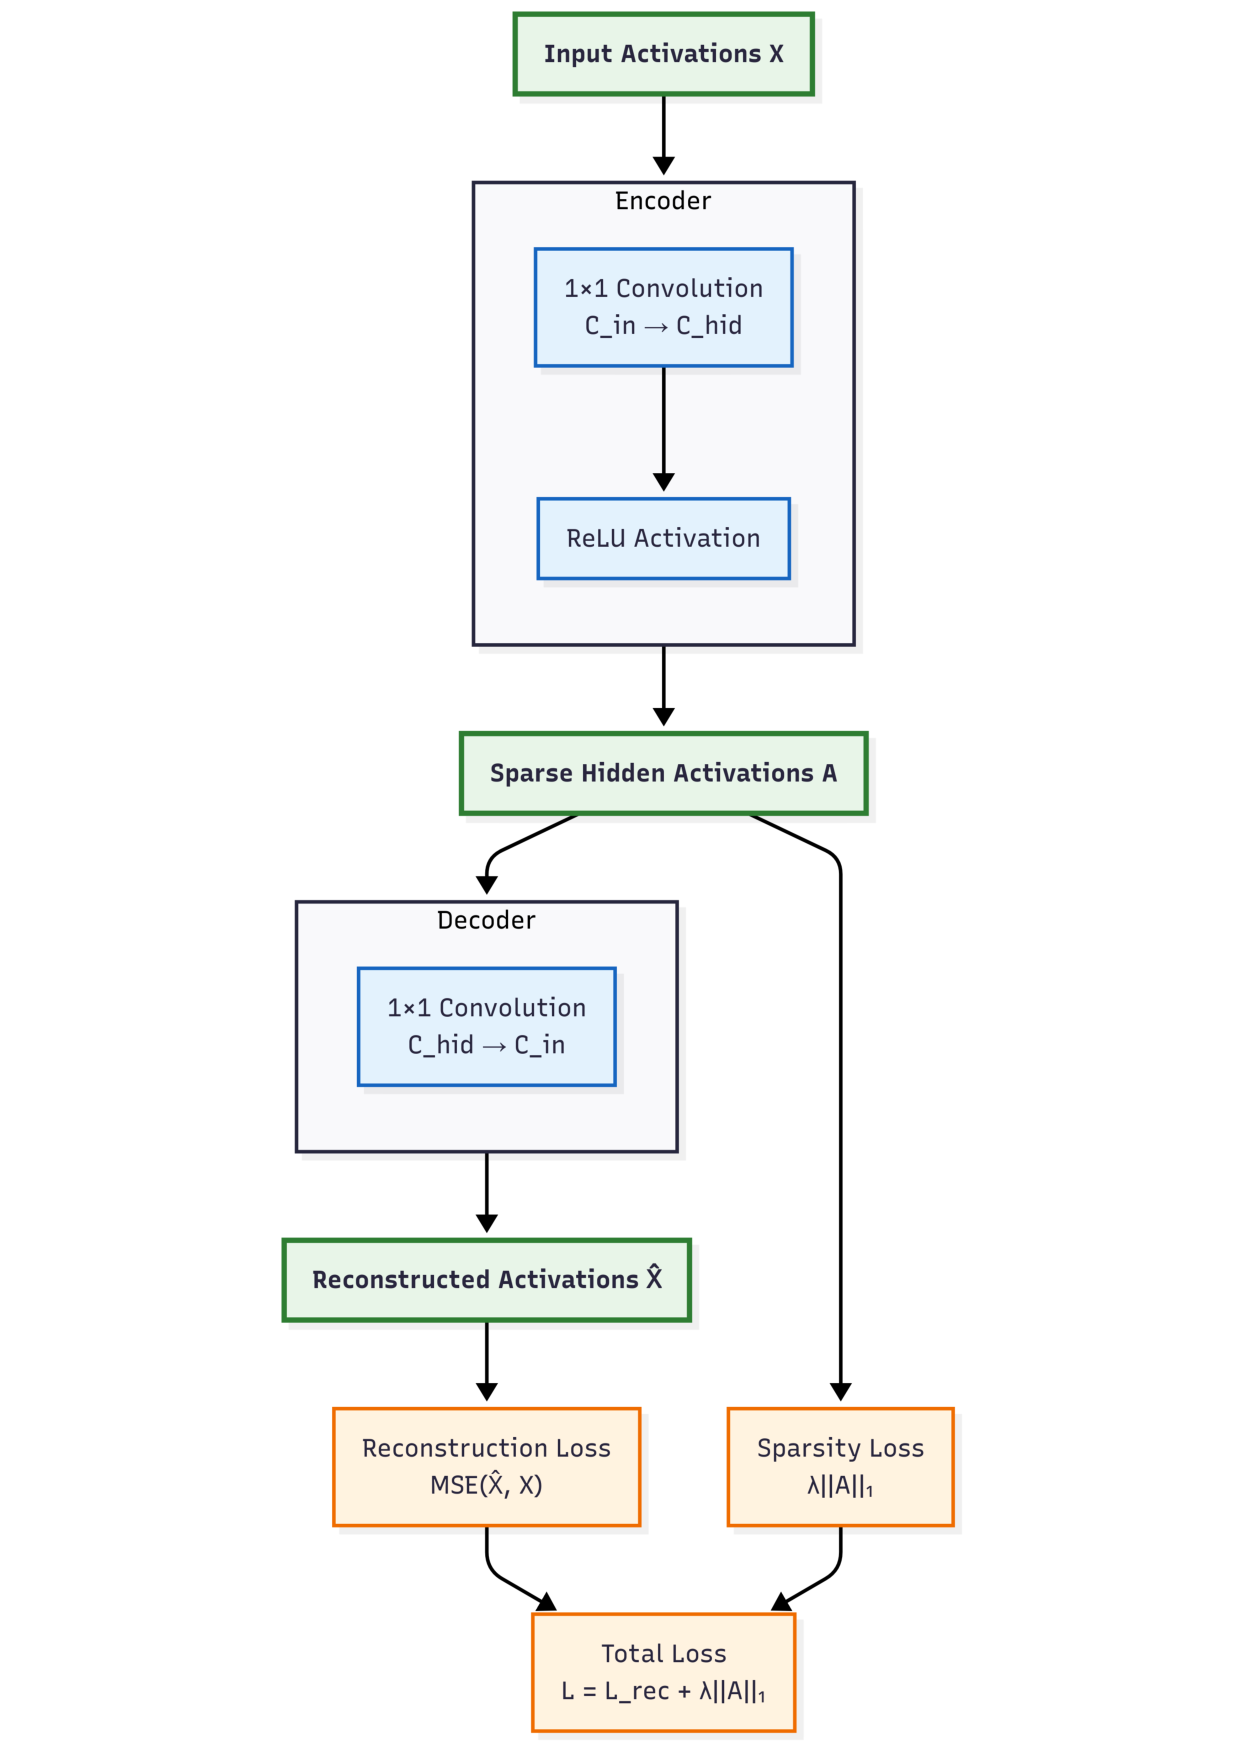
\includegraphics[width=0.8\textwidth]{figures/sae_mermaid.pdf}
    \caption{Sparse auto-encoder (SAE) architecture. An encoder applies a $1\times 1$ convolution and ReLU to map input activations $X$ to sparse hidden activations $A$; a second $1\times 1$ convolution reconstructs $\hat{X}$. Training minimises the reconstruction loss $\text{MSE}(X,\hat{X})$ plus an $\ell_{1}$ sparsity penalty $\lambda\lVert A\rVert_{1}$. \textit{Shapes:} $X\in\mathbb{R}^{B\times C_{\text{in}}\times H\times W}$, $A\in\mathbb{R}^{B\times C_{\text{hid}}\times H\times W}$, $\hat{X}\in\mathbb{R}^{B\times C_{\text{in}}\times H\times W}$.}
    \label{fig:sae_architecture}
\end{figure}

Recent approaches such as SAEs~\citep{bricken2023monosemanticity, gorton_2024_missing}, sparse probing~\citep{durrani2021transformer}, and neuron-level interventions~\citep{meng_2023_locatinga}, combat superposition by learning over-complete sparse dictionaries or low-dimensional subspaces that disentangle features and are discussed further in Section~\ref{subsec:post_hoc}. In particular, SAEs compress activations into sparse, over-complete features that split polysemantic neurons into monosemantic latents and have revealed interpretable features in both CNNs and transformers~\citep{conerly_update_2024}.


\subsection{Feature Visualization Techniques}\label{subsec:visualising_neural_networks}

Techniques such as those developed by~\citet{zeiler_2013_visualizing} represented the first work on interpreting the operations of deep neural networks. They employ a deconv-net, a model that maps feature activations from a deep layer back to the input pixel space by approximately reversing the network's pooling and convolutional operations. By reconstructing the maximally activating zones in pooling layers and being chained through subsequent CNN layers the reconstruction of complex visual representations of deep layers within the network can be achieved. This is normally very challenging due to the significant compression that is performed on the deep layers in the CNN. By applying this deconvolution the features appearing deeper in the network can be expanded back up to human interpretable scales.

Early work in understanding the functioning of neural networks focused on techniques that could visually represent the features that were encoded in the weights of the neural network. In particular, \citet{olah_feature_2017} developed techniques to generate maximally activating synthetic inputs that functioned as startlingly clear representations of channels and layers within the network. These visualisations revealed a clear hierarchy of abstraction, demonstrating how simple features from one layer (`curve-circuits') compose into more complex, semantically coherent representations (e.g., object parts) in the next. This work also demonstrated the use of gathering maximum activating samples from the training data and pairing it with particular channels and showing the similarity between these and the synthetically generated examples as a means of confirming the veracity of the visualisations.



While synthetic visualizations can be noisy, maximally activating patches, especially from within the environment, can yield interpretable results, confirming findings in~\citep{hilton_2020_understanding}. Work done on exploring SAEs trained on CNNS such as~\citep{gorton_2024_missing} makes effective use of visualisation to illustrate the improvement in interpretability of the SAE latents.


\subsection{Post-hoc Explanations}\label{subsec:post_hoc}
% Methods that explain already trained models
% Feature attribution, saliency maps, etc.

\subsubsection{Attribution and saliency methods} Post-hoc explanation methods aim to provide insights into already trained models without altering their architecture or training process. Examples include probing, SAEs, feature attribution methods (like LIME~\citep{ribeiro_2016_why}, SHAP~\citep{lundberg_2017_unified}), saliency maps~\citep{Simonyan14a,selvaraju_2017_gradcam}, and activation steering~\citep{turner_2024_steering,zou_2025_representation}.

LIME focuses on creating explainable functions by approximating a model's local behaviour around a specific input, and observing which changes create the greatest difference in the final outputs, weighting inputs by their proximity to the original input (with closer inputs being weighted more heavily). They then create a modified linear approximation that is explainable and train it on this weighted dataset which can then be more easily interpreted~\citep{ribeiro_2016_why}.

SHAP provides consistent estimations of feature importance based on Shapley values from cooperative game theory. It assigns each feature an importance value by calculating its average marginal contribution across all possible feature combinations, ensuring properties like local accuracy and consistency that other methods lack~\citep{lundberg_2017_unified}. It is quite costly to calculate however, as it requires calculating contributions over all possible feature subsets.

Saliency-based feature-attribution techniques, while originally developed for image classification, have been shown to yield insights into RL policies. These methods typically operate by computing the gradient of a relevant policy output (such as the value of a state or the probability of a specific action, $f(s)$) with respect to the input observation, $s$. The resulting saliency map is then defined as the magnitude of this gradient:
\[
    M(s) = |\nabla_s f(s)|,
\]
which highlights pixels that most strongly influence the agent's decision. Using this approach, \citet{greydanus_2018_visualizing} applied gradient saliency maps to Atari DQN agents, showing that agents frequently track critical entities like the ball in Breakout or enemy ships in Space Invaders (Figure~\ref{fig:breakout_saliency}).

\begin{figure}[htbp]
    \centering
    \includegraphics[width=0.9\textwidth]{figures/breakout_saliency.png}
    \caption{Saliency maps for a DQN agent learning to play Breakout, showing the evolution of attention patterns during training. Blue regions indicate areas most salient to the actor (policy), while red indicates areas salient to the critic (value function). Early in training, attention is diffuse; as learning progresses, the agent focuses on strategically relevant features such as the ball and the tunnel through the brick wall. Note that this figure illustrates saliency maps generally; the effect of longer rollouts on visualisation crispness discussed above is not shown here. Figure reproduced from~\citet{greydanus_2018_visualizing}.}
    \label{fig:breakout_saliency}
\end{figure}

To address the shortcomings of simple gradients, Sundararajan's integrated-gradients method\,\citep{sundararajan_2017_axiomatic}, which accumulates gradients along a path from a baseline input, was later extended to policy networks by~\citep{atrey_2020_exploratory}, who introduced `policy saliency' maps that operate over distributions of outputs from policy models. These approaches provide an easily computable and highly informative result without requiring additional training. However, unlike SAEs or steering vectors, these methods do not provide a mechanism for manipulating behaviour.

\subsubsection{Probing}\label{subsubsec:probing}
Perhaps the most famous and enduring of post-hoc techniques is probing, particularly the linear probe~\citep{alain_2018_understanding}. This is simply a linear classifier trained on activation data from a given layer on target labels that are provided based on a pre-registered target of interest. The degree of accuracy that the probe can achieve represents the degree to which a given layer can be said to contain a representation of the given target feature within the layer~\citep{alain_2018_understanding}. Deeper probes consisting of multiple layers are also a useful tool, but these can obfuscate the degree to which the target feature is actually present due to the additional computation being performed.

Probing is a core tool in mechanistic interpretability due to the wide array of situations where it can be applied and the low cost of implementation. It also reveals a great deal of information about where in the network a certain operation is being performed such as object detection, spatial reasoning, or feature composition. 

Probes have been able to provide powerful insight when applied creatively to neural networks. An excellent example of the explanatory power of probes can be found in~\citet{li_2024_emergent} which demonstrated that a model trained to produce legal moves in the game of Othello after being provided a preceding sequence of moves had a rich encoding of the board state embedded within the weights, as opposed to having learned complex heuristics to predict likely next moves. They demonstrated using non-linear probes (2 layer MLPs), that they could extract the state of the board by which types of piece occupied each square on the grid. They did this by training 64 probes in parallel, each probe being trained exclusively on the underlying ground truth data for a specific grid position across the training datasets. The ground truth data consisted of `black', `white', or `neutral' states for each position. They tried linear probes and the 2 layer probes, and found that the linear probes were able to achieve only around 20\% performance while the 2 layer probes achieved up to 98.7\% accuracy.~\citet{nanda_2023_emergent} expanded on this work by showing that in fact it was possible to achieve extremely high accuracy with linear probes, but that the ground truth data needed to be altered to represent `yours', `mine', or `neutral', and that it would swap depending on whose turn in the game it was. This demonstrated that the additional computation performed by the 2 layer probes was obfuscating the underlying representation that the model had learned.

However, probes do have significant limitations as well. They provide only correlational evidence of the purpose of what the network is doing. They may show that some activation contains the relevant information but not what it is doing with it or whether it is acting upon it. There is also a risk that probes are in fact doing computational work to construct features rather than simply revealing them, if the probes have multiple layers and many neurons. For example, an MLP probe trained to detect the presence of a cat in activation space could infer the cat from isolated features in the network that would normally only be combined later in the network. The Othello GPT example illustrates how the MLP probes were performing additional computation to adjust to the non-native representation of the board state within the activations.


\subsubsection{Sparse Probing}

Sparse probing is an approach that aims to address polysemanticity (Section~\ref{subsec:superposition}) by selecting a portion of a network, such as a channel, a layer, or multiple channels, and then training a linear classifier that uses only a subset of size $k$ neurons from that section to predict a target feature~\citep{gurnee_2023_finding}. The classifier makes predictions about the target class using only these $k$ neurons, and researchers can then observe which neurons have the highest predictive power by comparing classification accuracy. By iteratively selecting different values of $k$ and retraining, this method surfaces which neurons are most important for feature detection, and allows researchers to determine how much of the network is required for the given operation based on the accuracy scores for different sizes of $k$.

When $k=1$, this method isolates individual neurons that serve as feature detectors. Experiments across diverse architectures and tasks revealed that certain high-level semantic features achieve classification accuracies exceeding 75\% using single neurons. 
The existence of neurons with near-monosemantic responses indicates that neural networks can develop localized representations despite their distributed architecture. This localization appears most pronounced in middle layers, where abstract representations have formed but have not yet been transformed into task-specific outputs. Such neurons enable targeted interventions and provide empirical evidence that understanding can be done through analysis of individual components rather than requiring more complex distributed interventions.

Feature detection accuracy exhibits a characteristic non-monotonic pattern when varying the sparsity parameter $k$: rapid improvement for small $k$ followed by plateau or decline~\citep{gurnee_2023_finding}. This pattern indicates encoding through a small core set of highly informative units, with additional units contributing marginally or detrimentally to classification. Optimal sparsity varies systematically with feature complexity and network depth. Early layers involved with integrating low level features typically require $k\in[10,50]$ before yielding high accuracy, while later layers can peak with $k\in[1,10]$.

Sparse probing has significant limitations in that it requires significant human effort to determine the nature of the features detected with the sparse probing, and thus the field has not moved much in this direction, with unsupervised dictionary learning approaches such as SAEs becoming the preferred approach for isolating features in the network. However, sparse probing still provides significant utility in understanding smaller networks where the number of features is much fewer and target concepts can be concretely specified for probe training and especially allows for concrete understanding of the precise operations of the actual network that may be obfuscated in an SAE.

\subsubsection{Dictionary learning}\label{subsubsec:dictionary_learning}

Dictionary learning~\citep{olshausen_1996_emergence} provides a principled approach to resolving superposition (Section~\ref{sec:interpretability}). The goal is to discover an overcomplete dictionary $D \in \mathbb{R}^{d \times k}$ (where $k > d$) whose columns serve as basis vectors that can represent input data $x \in \mathbb{R}^d$ through sparse linear combinations:
\[ x \approx D \cdot \alpha, \]
where $\alpha \in \mathbb{R}^k$ is a sparse coefficient vector. Unlike standard bases that require exactly $d$ linearly independent vectors, dictionary learning trades redundancy (overcomplete basis) for sparsity (each data point activates only a few basis vectors). This sparse, distributed representation disentangles features that would otherwise be superposed in the original $d$-dimensional space, as described by Equation~\ref{eq:superposition}.

Classical algorithms such as K-SVD~\citep{aharon_2006_ksvd} and FISTA~\citep{doi:10.1137/080716542} solve this optimisation problem through iterative sparse coding and dictionary updates. SAEs provide a neural network approach to this same objective.

\subsubsection{Sparse AutoEncoders}\label{subsubsec:SAEs}

SAEs utilise neural networks to perform unsupervised discovery of the dictionary. This provides a sparse encoding of the original features of the model (which we refer to as latents in the SAE), which arise due to the enforcement of a sparsity penalty applied during the training of the SAE. SAEs aim to faithfully reconstruct the activations of a given layer in a network while keeping their own internal activations sparse. The training objective is therefore to find encoder and decoder weights that minimise a loss function combining a reconstruction term and a sparsity term, which typically takes the form:
\[L(x) = \|x - \text{Dec}(\text{Enc}(x))\|_2^2 + \lambda \|\text{Enc}(x)\|_1\]
Here, \(x\) represents the original activation from the base model, the L2 norm penalizes poor reconstruction, and sparsity is enforced by minimising the product of the L1 norm of the SAE's internal activations, and a coefficient \(\lambda\)\citep{bricken2023monosemanticity}.  

SAEs typically learn an overcomplete basis, where the hidden layer of the SAE is much larger than the original layer it is reproducing, typically chosen by multiplying the original hidden dimension size by some expansion factor. This high dimensionality allows the SAE to represent the input activations using a small number of highly specific, disentangled features. This addresses the problem of polysemantic `units' in a model, which can make the task of accurate interpretability much more challenging~\citep{elhage2022superposition}.

The direct methodological precedent for applying SAEs to convolutional networks comes from recent work by \citet{gorton_2024_missing}, who successfully trained SAEs on the InceptionV1 image classifier. Their approach uses a `1x1-conv SAE' architecture, as illustrated in Fig~\ref{fig:sae_architecture}. An encoder with a learnable $1\times1$ kernel maps the input activation tensor $X$ to a sparse, high-dimensional hidden activation tensor $A$, which a symmetric $1\times1$ decoder then uses to reconstruct $\hat{X}$. To train this effectively on CNNs, they introduced several key innovations. First, to manage computational cost, they used \emph{activation oversampling}, preferentially sampling training data from spatial locations with high activation magnitudes to focus on learning meaningful features rather than background noise. Second, they used highly over-complete dictionaries, with expansion factors up to 8, to provide the capacity needed to disentangle features. The results were compelling: their SAEs successfully split known polysemantic `double-curve' units in InceptionV1 into distinct monosemantic features and recovered a suite of previously `missing' curve detectors. These findings provide concrete evidence that dictionary-learning SAEs can resolve superposition in CNNs and motivate their application to RL agents with convolutional backbones.

To formalise the above concept, let $a^{l}(x)\in\mathbb{R}^{d}$ be the activations of layer $l$ for input $x$, and let $w\in\mathbb{R}^{d}$ be the extracted weight vector of the linear classifier trained to distinguish positive concept examples from counter-examples.  We take the concept activation vector as
\[
    v^{l}_{C}= \frac{w}{\lVert w \rVert_{2}}.
\]
Following~\citet{gorton_2024_missing}, the extent to which concept $C$ influences the logit $f_{k}(x)$ for class $k$ is measured by the directional derivative
\[
    S_{C,k,l}(x)= \nabla_{a^{l}(x)} f_{k}(x) \cdot v^{l}_{C},
\]
whose sign indicates whether amplifying the concept increases ($S_{C,k,l}>0$) or decreases ($S_{C,k,l}<0$) the likelihood of a particular prediction.

Because these can be learned with a lightweight linear probe and then used to potentially intervene on neural network activations as illustrated in work such as Othello GPT~\citep{nanda_2023_emergent}, this technique has become fundamental as a tool in alignment~\citep{meng_2023_locatinga}, and lays a conceptual foundation for things like steering vectors, which are produced in a different way but share many properties~\citep{turner_2024_steering}.


The feature visualization methodologies discussed, such as synthetic visualization (optimizing an input image for maximal channel activation) and finding maximally activating dataset samples~\citep{olah_feature_2017,hilton_2020_understanding}, are also forms of post-hoc analysis.


\subsubsection{Concept Activation Vectors} 
Concept Activation Vectors (CAV) provide a way to bridge the gap between the high dimensional vector space of neural network activations and human-understandable concepts. To construct a CAV for a concept (`striped'), one collects a small set of images that exhibit the concept and a set of random counter-examples, records the activations from a chosen layer, and trains a linear classifier to separate the two groups. The normal vector to the resulting decision boundary is the CAV. This can then be manipulated in one direction or the other to produce more or less of the effect you desire~\citep{kim_2018_interpretability}. This can be used to test how much a particular concept is relied upon when the network is making a prediction. Recent applications of CAVs have shown promising results in debugging vision models and identifying spurious correlations in training data.

\subsubsection{Activation Steering}\label{subsubsec:activation_steering}
Activation steering, as demonstrated in~\citet{mini_2023_understanding,turner_2024_activation} discussed further in Section~\ref{sec:Understanding}, is another post-hoc technique. Steering typically makes use of CAVs, captured by using the difference in activations between states with and without a particular characteristic, can be used to influence a policy model's behaviour by acting as a superstimulus for particular environmental aspects. This is achieved through the transformation $h^{l'} = h^l + \alpha \cdot v^l$, where the steering vector $v^l$ is added to the original activations $h^l$, with $\alpha$ modulating the intervention strength. The steering vector itself is computed as $v^l = \mathbb{E}[h^l|\text{with target}] - \mathbb{E}[h^l|\text{without target}]$, capturing the difference in activations when the target is present versus absent.

In language models (LMs) a typical approach used to do activation steering is to use contrastive pairs~\citep{turner_2024_activation}. In this approach one presents two different segments of text that are identical in every way except one, for example one may pass the following two inputs through an LM and then calculate the mean across the activations of the tokens and then calculate the difference in the two mean values to capture the `speak in French' concept vector, which can then be used to steer the model to speak in French or English by modifying $\alpha$ to be positive or negative and adjusting its magnitude. This is normally done across many samples, with the mean of those pairs being used for steering. 
\begin{itemize}
    \item \textbf{English:} ``The teacher explained the complex problem using simple examples.''
    
    \item \textbf{French:} ``L'enseignante a expliqué le problème complexe en utilisant des exemples simples.''
\end{itemize}

Activation steering is an excellent tool for interpretability due to the ease and speed with which it can be used, and because it allows researchers to immediately observe how a network responds to a specific concept being made more or less prominent in the forward pass of the network. They also allow researchers to determine whether a concept exists and is easily representable in given layer of a network. Given that you can extract concept from single layers, or multiple layers simultaneously, one can test whether the concept is meaningful within a certain part of a network by the degree of change in output observed by its application there.

\subsection{Intrinsically Interpretable Models}\label{subsec:intrinsic}
Intrinsically interpretable models are designed from the outset to be understandable, often by constraining their complexity (e.g., linear models, decision trees) or by building in mechanisms that are inherently transparent. Training SAEs can be seen as an effort to transform parts of a complex model into a more intrinsically interpretable representation by disentangling features.

Many existing interpretability techniques were developed for supervised settings with i.i.d.~data. Reinforcement learning violates many of these assumptions. For example, observations are generated by an agent acting in, and affecting, a dynamic environment, and credit must be assigned across time. As a result, many tools require adaptation to work within this paradigm. The next section explores some techniques that have been developed explicitly to overcome this gap.

\subsection{Causal Methods in Interpretability}\label{subsec:causal}

Many of the techniques discussed in the methodology, such as activation steering (Section~\ref{subsubsec:activation_steering}), can serve dual roles as both post-hoc explanation tools and causal testing methods when applied systematically. This section focuses on additional causal techniques and frameworks for rigorous causal claims in interpretability research. These techniques actively modify the operations of the network, testing whether specific components are genuinely responsible for behaviours of interest~\citep{10.5555/1642718}.

Modern systematic ablation has evolved through several generations. Zero ablation, the simplest approach, sets components to zero but can lead to out-of-distribution behaviours since networks rarely encounter zero values during training. Mean ablation, which replaces components with their average values across a sample dataset, better preserves activation statistics but may incompletely remove information if the mean itself carries useful information. Recent work~\citep{li_2024_optimal} introduces optimal ablation constants that are computationally determined to minimise the expected loss on the task, reducing the amount of distributional shift in the final outcome.

Work on finding induction heads in neural networks~\citep{olsson_2022_incontext} is a prime example of rigorous systematic ablation. In this work they thoroughly demonstrated causality via targeted removal. Their task setup involved identifying how LMs were able to successfully complete simple A-B pattern matching, meaning that when a pattern of B following from A was observed the model should repeat this pattern when a later example of A was shown. When induction heads were ablated in small models, in-context learning collapsed from near-perfect to near-random on the task of A-B pattern matching. This showed that induction heads were essential for this task.

For agents with spatial convolutional representations, targeted synthetic interventions can directly test the functions of parts of the network by intervening on their values directly.~\citet{mini_2023_understanding} demonstrated that clamping a single activation in a channel that typically identified the location of the cheese (channel 55) to a large positive value at a specific location in the maze could steer the agent to that location, as if that was the final goal of the maze. This provided direct causal evidence that this channel had an unusual ability to steer the direction of the agent.

These causal techniques provide the foundation for the experimental methodology employed in this thesis. Systematic ablation is used to test the necessity of individual SAE channels for navigation (Section~\ref{sec:expanded_ablation_methodology}), while activation interventions combined with behavioural testing establish sufficiency of specific channels for steering agent behaviour (Section~\ref{subsubsec:steering_interventions}). Together, these approaches move beyond observation to establish genuine causal mechanisms underlying goal representation in RL agents.


\section{Interpretability in Reinforcement Learning}\label{sec:rl_interpretability}

Interpretability in RL presents unique challenges due to the agent's interaction with an environment, the fact that specific outputs of the model might be extremely semantically distant from the contents of a given activation, and because we can only infer the meaning of a given observation of an activation within the model, we can't directly glean it as we could a word extracted from the embedding space of a language model.

Recent research shows that such models naturally learn geographic mappings of the world related to locations that can be retrieved directly from the activations of the network, effectively building simplified world models~\citep{gurnee2023language}. Similarly, analyses of agents trained on complex games like chess demonstrate that these systems acquire human-understandable strategic concepts, such as piece values or tactical motifs, purely from self-play~\citep{mcgrath_2022_acquisition}. These findings suggest that the internal workings of these models are richer than previously thought and lend support to the idea that they plausibly learn to represent goals that can be directly extracted from the model and understood. As illustrated in Figure~\ref{fig:environment-overview}, even a seemingly simple maze can embed multiple, dynamically changing goals whose representations the agent must learn to use effectively.

Work by~\citet{betley_2023_localizing} found a specific circuit in the convolutional layers of the Impala model that activated strongly when the direction to go was `up' and didn't activate when the goal was in a similar position but the agent would need to go in a different direction. This indicates that much of the `planning' was already performed in the CNN layers, suggesting it should be possible to train probes that can detect the exact direction the agent needs to move towards.

Work exploring the Procgen Coinrun environment builds on saliency based methods (Section~\ref{subsec:post_hoc}) to calculate an attribution within the model weights themselves. By measuring the contribution of a given convolutional feature map to the value function, it becomes possible to determine if a particular feature that the model is observing is likely to have a positive or negative effect on the success of the model, based on whether the collected gradient multiplied by the activation score is positive or negative. This advances previous saliency mapping methods by linking the gradients to specific features within the model, rather than pixels in the input~\citep{hilton_2020_understanding}.

This is achieved by applying non-negative matrix factorisation (NMF) of the attribution tensor to cluster correlated locations across channels into object-level `features' such as coins, enemies, obstacles etc. By using this dimensionality reduction they are able to produce clear, interpretable object detectors. 



% To provide a precise explanation of this process, let $X^{(n)}\in\mathbb{R}^{C\times H\times W}$ be the activation tensor of a convolutional layer for input $n$ and let $V^{(n)}$ be the value head.  Element-wise product of activation and gradient attribution is
% \[
% A^{(n)}_{c,h,w}=X^{(n)}_{c,h,w}\;\frac{\partial V^{(n)}}{\partial X^{(n)}_{c,h,w}}.
% \]
% Flatten $A^{(n)}$ to a vector $a^{(n)}\in\mathbb{R}^{D}$ with $D=CHW$ and stack $N$ such vectors into a matrix $R\in\mathbb{R}^{N\times D}$. This results in an $N \times D$ matrix where each row is a single observation, and each column is a `feature location'. We then apply NMF to this matrix, keeping $A^{(n)+}_{c,h,w}=\max\bigl(0, A^{(n)}_{c,h,w}\bigr)$ to satisfy the non-negativity constraint. Non-negative matrix factorisation seeks
% \[
%     R\;\approx\;W H,\quad W\in\mathbb{R}_{\ge0}^{N\times r},\;H\in\mathbb{R}_{\ge0}^{r\times D},
% \]
% with a small rank $r$. Each row of $H$, reshaped back to $(C,H,W)$, yields a sparse mask that acts as a detector for in-game entities (coin, enemy, hazard). 



\section{Understanding and Controlling a Maze Solving Policy Network}\label{sec:Understanding}
Previous work by~\citep{mini_2023_understanding} demonstrated the ability to manipulate an agent's navigation in a simple maze environment with an intervention to a single channel in the network, providing the primary motivation for this work with the intent of extending these techniques to more complex multi-objective settings. The work specifically used an agent which had been trained in a modified version of the environment where the cheese was only ever added to the top right of the environment, and then deployed the agent into settings where the cheese could spawn at any location in the maze. This meant that there was a tension between the agent's natural tendency to want to go to the top right of the environment and to go the cheese location.

They go on to show that the agent's decision making about whether it travelled to the top right or towards the cheese alone was determined by both the Euclidean distance between the agent and the cheese and the path distance between the agent and the cheese. This means that the agent had multiple separate mechanisms driving its decisions rather than being a single unified policy. They did this by showing through regression analysis that if the agent was an equal path distance from two instances of cheese, it would tend to approach the cheese that was also closer in Euclidean distance. 

This shows a surprising contradiction in the agent because Euclidean distance should not meaningfully affect a maze-solving policy (the agent cannot walk through walls), suggesting the agent is not relying on a single reward-maximising policy but is instead operating under multiple competing goals.

They further demonstrate that neural networks can develop interpretable mechanisms to track goals. The authors identified specific channels that tracked the location of objectives in a maze environment and showed that these could be manipulated to control the agent's behaviour. They found that steering vectors, the difference in activations between otherwise identical states with and without an entity, could be used to influence the model's behaviour in predictable ways. This work serves as the foundation for our research, though we extend it to a multi-objective setting.

Recent concurrent work by~\citet{trim_2024_mechanistic} extends the work done by~\cite{mini_2023_understanding} to analyze goal misgeneralization. Their layer-by-layer analysis reveals a hierarchy of representations: early layers (b1.conv) detect basic features such as walls, paths, and the cheese goal; middle layers develop more abstract concepts including possible `flood fill' patterns for directional pathways; while deeper layers create highly abstracted representations where identifying the goal becomes challenging. They further confirm the positional bias seems to exist regardless of the position of the final goal within the maze, indicating a deeply learned tendency towards this direction, rather than the result of a perceptual error.

\subsection{Discovering and Controlling Goal Representations}
The authors successfully isolated the network's representation of the `cheese' goal and demonstrated causal control over the agent's behaviour. First, they defined a `cheese vector' by taking the difference in mean activations at a specific layer between trajectories where cheese was present and those where it was not:
\[
v_{\text{cheese}}^{l} = \mathbb{E}_{s \sim \text{traj}_{\text{cheese}}}[\text{act}^{l}(s)] - \mathbb{E}_{s \sim \text{traj}_{\text{no-cheese}}}[\text{act}^{l}(s)]
\]
Adding this vector back into the network's forward pass, scaled by a coefficient $\alpha$, allowed them to controllably amplify or suppress the agent's cheese-seeking behaviour.

Their most significant contribution was demonstrating this control causally through \emph{activation patching}. They intervened on the final convolutional layer of the policy network by copying the activation pattern from a small spatial region of a channel corresponding to a real cheese location and `pasting' it into the same channel at a different, empty location. By doing this they could reliably steer the agent to the empty location as if the cheese were there.

This effect was highly localized. They identified that out of 16 channels in the layer, just 11 were responsible for this behaviour. Ablating these "cheese channels" destroyed the agent's ability to find the cheese, while leaving other navigational capabilities intact. This proves that goal representations can be sufficiently modular and concentrated to allow for targeted manipulation, motivating the use of more advanced techniques like SAEs to further dissect these representations in a more complex, multi-objective setting.


\section{Gaps in the Literature}\label{sec:gaps}
Prior to the research detailed in the accompanying papers, several areas in RL interpretability remained open for exploration:

\begin{itemize}
    \item Understanding how RL agents track and switch between multiple objectives, especially when those objectives are not the immediate next target.
    \item The application and efficacy of techniques like SAEs for disentangling representations specifically within RL agent architectures, particularly CNNs.
    \item Investigating how different aspects of neural network activation encode useful information for the next layer such as how activation strength within a channel might encode information like entity identity.
    \item The role and potential utility of `dead' channels in SAEs for interpretability, which cease to activate during normal operation but might retain learned decoder weights.
    \item The generalisation of interpretability findings from simpler RL agents to more complex architectures like decision transformers or RNN-based agents, especially for tasks requiring memory.
\end{itemize}

\section{Summary}\label{sec:lit_summary}
Prior work shows huge potential in the applications of RL agents due to their ability to achieve superhuman performance generalise broadly. However, the opacity of how this is achieved represents a persistent problem. A resurgence of interest in this area due to its application in frontier AI models adds urgency to better understand these models and how they operate on a mechanistic level~\citep{mini_2023_understanding,hilton_2020_understanding}. Techniques such as activation analysis, steering vectors, and feature visualization have provided initial windows into these systems. However, challenges like polysemanticity (where neurons or channels respond to multiple unrelated concepts~\citep{olah_2020_zoom,elhage2022superposition}) and the distributed nature of representations often make it challenging to make strong conclusions about the operation of the neural network.

The application of tools like Sparse Autoencoders offers a potential solution for being able to make confident statements about whether the nature of how models truly learn to encode concepts~\citep{elhage2022superposition,bricken2023monosemanticity}, potentially making the functional roles of different network components clearer. While much of the early MI work focused on LLMs, applying and adapting these techniques to RL, with its emphasis on clear goals and environments with fewer components and potentially broadly generalisable solutions offers the ability to make unique insights that may apply to ML models more broadly.

The research presented in the accompanying papers (forming the basis of this thesis) builds directly on this existing work by:
\begin{itemize}
    \item Extending activation steering and intervention techniques to more complex, multi-objective RL environments like Procgen Heist.
    \item Applying Sparse Autoencoders to the convolutional layers of an RL agent to disentangle features and investigate the extent to which multiple entities are truly captured within a single layer of the model and through what mechanism this is done. 
    \item Systematically analyzing the role of individual channels in navigation and goal pursuit through methods like ablation studies and retargeting interventions.
    \item Exploring novel mechanisms of information encoding, such as multiplexing entity information within a single channel through varying activation strengths.
\end{itemize}
These contributions aim to deepen our understanding of how RL agents represent and pursue goals, and to refine the tools available for mechanistic interpretability for use in this domain.

\chapter{Methodology}
\label{ch:methodology}

\section{Environment and Model}
\label{sec:env_model}
    \subsection{The Procgen Heist Environment}
    \label{subsec:heist_env}
    The Procgen Heist environment, from the suite of procedurally generated environments by \citet{cobbe_2020_leveraging}, was chosen for this research. The agent's objective is to navigate a maze to collect a gem, which may require first collecting up to three keys (in the fixed order of blue, green, red) to open corresponding locks. The environment's procedural generation varies the maze layout and the number of key-lock pairs present in each episode, from zero to three.

    This environment provides a sparse reward signal, with a reward of +10 for reaching the gem and 0 otherwise. This design, coupled with the variable difficulty, establishes a natural curriculum that allows agents to succeed with random exploration in simpler levels before developing a more sophisticated policy.

    The choice of a Procgen environment is motivated by the need to learn generalizable representations. The procedural nature of the mazes discourages the agent from memorizing simple heuristics and instead promotes the development of robust internal models of entities and game mechanics. Furthermore, Heist's multi-objective nature is expected to produce complex internal behaviors, such as general-purpose navigation circuits that can be dynamically retargeted based on the current goal.

    For this investigation, the `easy' distribution of the environment was used, which provides the full 64x64 observation to the agent, making the environment a fully-observable Markov Decision Process (MDP). While memory-based, partially-observable variants exist, they were not used. The distribution of entities is noteworthy: since levels are sampled uniformly from all configurations, the gem and the blue key/lock appear more frequently than the green and red pairs.

    \subsection{Model Architecture}
    \label{subsec:model_arch}
    We train a compressed version of the Impala model that uses 5 convolutional layers instead of 15 as used in the original Impala paper. This architecture comes from~\cite{hilton_2020_understanding} where they find that this model was more interpretable with no discernible loss in performance. We include the model architecture in full in Appendix~\ref{app:model_architecture}.

    When training our model we use a simple PPO implementation from an open source implementation designed to train Procgen models called Procgen-pfrl. We used the easy distribution of the environment due to compute limitations. We tested model training over a number of different batch sizes and distributions. The model checkpoints used to derive our main findings were trained with standard hyperparameters: learning rate 5e-4, 64 parallel environments collecting 256 steps each (16,384 total steps per update), processed in batches of 8 over 3 epochs for 800 million steps. The training dynamics were significantly impacted by changes to batch size often completely collapsing training performance, but over the course of 5 runs with separate seeds with the parameters above we were able to replicate similar model dynamics in each case. 
    \subsection{Model Training}
    \label{subsec:model_training}
    The policy models were trained using Proximal Policy Optimization (PPO) with an open-source implementation based on PFRL, specifically designed for Procgen environments. We also made use of Envpool to accelerate the speed of our training while keeping the actual training dynamics unchanged\cite{weng2022envpool}. Training was conducted until convergence, which in this case was when no statistical improvement was observed for 10000 update steps. The primary model was trained for approximately 600 million steps. 

    To explore the effects of training dynamics on the final learned representations, experiments were run with different training configurations. These variations primarily involved altering the batch geometry through four main hyperparameters: the number of parallel environments, the number of steps per rollout, the mini-batch size, and the number of epochs.


    In the primary configuration reported in this thesis, we used a setup of ($N_{\text{env}}=64$, $N_{\text{step}}=256$, $\texttt{batch\_size}=8$, $n_{\text{epoch}}=3$). In this geometry, the rollout buffer contains $N_{\text{env}}N_{\text{step}}=16\,384$ transitions. This is reshaped into $8$ mini-batches, each containing $B_{\text{mb}}=2\,048$ samples. The optimizer performs $8\times 3 = 24$ gradient steps per PPO update, processing a total of $16\,384\times 3 = 49\,152$ sample-updates per cycle. This configuration was chosen to balance stable learning from large batches with reasonable training time per update.

    We ran 5 sets of training runs for this geometry in order to confirm the repeatability of our results, and ran further training runs with other geometries to observe the extent to which this altered  the final structure of the model weights. Namely ($N_{\text{env}}=128$, $N_{\text{step}}=128$, $\texttt{batch\_size}=8$), ($N_{\text{env}}=256$, $N_{\text{step}}=256$, $\texttt{batch\_size}=8$), and ($N_{\text{env}}=256$, $N_{\text{step}}=128$, $\texttt{batch\_size}=16$). These variants were included to probe the sensitivity of the learned representations to rollout length and batch composition. A detailed comparison of the models trained under these settings is provided in Chapter~\ref{ch:results}.

\section{Interpretability Techniques Employed}
\label{sec:interp_techniques}

\subsection{Feature Visualization}
    \label{subsec:feature_viz}
    A useful initial approach involved simply creating direct visualiations of the convolutional layers of the model. This involved simply taking a given layer and applying a colour spectrum according to the strength of the activations within that region of the grid. This approach, following~\cite{mini_2023_understanding}, provided a direct view of which spatial regions triggered strong positive or negative responses in different channels. Figure~\ref{fig:filter_visualizations} shows an example of this visualization technique applied to multiple layers.


    \begin{figure}[ht]
        \centering
        \begin{tabular}{cccc}
        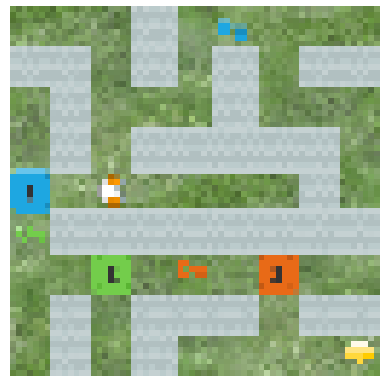
\includegraphics[width=0.25\linewidth]{figures/observation.png}&
        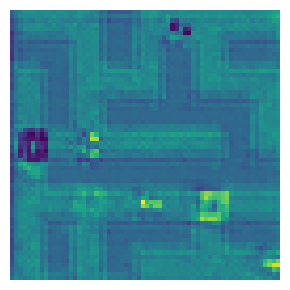
\includegraphics[width=0.25\linewidth]{figures/layer1_filter10.png}&
        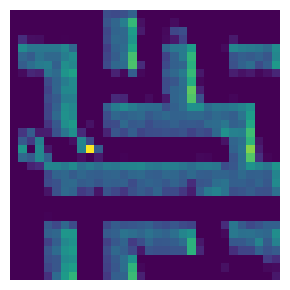
\includegraphics[width=0.25\linewidth]{figures/layer2_filter10.png}&
        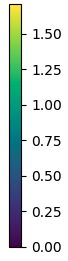
\includegraphics[width=0.067\linewidth]{figures/colorbar.png}
        \end{tabular}
        
        \vspace{0.5em}
        
        \begin{tabular}{ccc}
        \hspace{0.1725\linewidth}&
        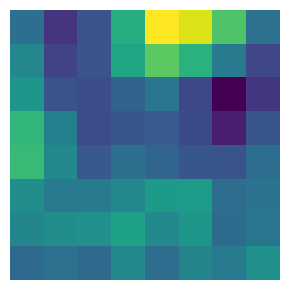
\includegraphics[width=0.25\linewidth]{figures/filter29_layer8_no_title.png}&
        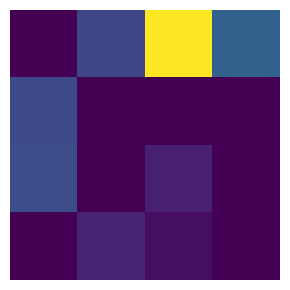
\includegraphics[width=0.25\linewidth]{figures/filter29_layer9_no_title.png}
        \end{tabular}
        
        \caption{Visualization of the maze and neural network activations in different layers. Top row (left to right): 
        observation input, layer 1 channel 10, layer 2 channel 10, and activation colorbar. 
        Bottom row: layer 8 channel 29 and layer 9 channel 29. In the top row filters we observe a minimal activation around the regions of the blue key and lock and in the bottom row we see maximal activations around the blue key. This is a replication of the approach used by\cite{mini_2023_understanding} in order to get an initial sense of the clarity with which entities could be seen in activations.}
        \label{fig:filter_visualizations}
    \end{figure}

    \subsection{Comparative Activation Analysis}
    \subsubsection{Parallel rollout analysis}
    A key question that this research aimed to tackle is how the network determines which entity to target next, as there are many instances where there are multiple routes leading to different entities in the environment, and the sequence of collection is critical to success.

    To directly compare the model activations when targeting different entites, a simple toy maze environment was created that would test some basic capabilities in the model, specifically its ability to turn a corner and travel in a straight line towards a target. The maze took the shape of a T junction, with the agent started at the middle point, and with a blue key placed in the bottom right. A visual of the maze is provided in Figure. A rollout of the policy was then performed, but for each step of the rollout, the environmental state was modified to produce an observation with the gem, blue key, green key, and red key. By doing this at every step, 4 parallel rollouts with different entities were produced which allows for a perfectly controlled experiment from which we could observe the variations in activation patterns based only on the nature of the target entity. 
    
    With these rollouts we then tracked both the mean centered activation values for each entity, as well as the raw activation magnitudes across all channels in layers conv3a and conv4a. The mean-centering was performed by computing each channel's temporal mean across the entire trajectory and subtracting this mean from the activation at every timestep. This transformation centers each channel's activations around zero, removing baseline offsets between channels and making temporal dynamics comparable across channels with different baseline activation levels. Both raw and mean-centered activations were recorded to enable analysis of absolute activation strengths as well as relative temporal patterns. This design isolates the effect of entity type on the model's internal representations while holding agent position, maze geometry, and navigational requirements constant across all four parallel trajectories.
    

    \begin{figure}[H]
        \centering
        \includegraphics[width=0.7\textwidth]{figures/entity_trajectories_grid.pdf}
        \caption{This illustrates the parallel rollout of the agent, with each step taken by agent remaining exactly the same while we create an observation with each of the blue key, green key, red key, and gem.}
        \label{fig:intervention-experiment}
    \end{figure}

    

    \subsubsection{Activation Ranges Per Entity Collection}
    Because the previous experiment only includes a single entity, and not the full set of entities that the network would typically see, it provides limited insight into the activations during an actual rollout. To observe shifts in patterns that would be closer to the distribution of observations the network was trained on, and to capture how the presence of the other entities affects the activation patterns. To do this we used a simplified cross-maze environment containing the keys and the gem and no locks, and observing the differences in activations over the course of a rollout, while noting the timesteps at which different entities were collected. We used this environment because it provides little in the way of navigational challenges, and also makes it possible for the agent to go towards any of the entities, meaning we can test its natural preference ordering more simply. We also remove any confounders that may arise from specific maze patterns.

    \begin{figure}[H]
        \centering
        \includegraphics[width=0.9\textwidth]{figures/cross_maze.png}
        \caption{This illustrates the cross maze used for analysing the sequential entity collection activations. The positions of the entities is randomised in any given run in order to avoid creating a bias in the observed activation patterns.}
        \label{fig:cross_maze}
    \end{figure}



    \subsection{Sparse Autoencoder (SAE) Training}
    \label{subsec:sae_training}
    SAEs are a type of unsupervised learning technique that can be used to break down the most critical functions of a model into a more interpretable set of sparse latents, often by training an overcomplete basis on the original activations of a given layer of the network~\cite{bricken2023monosemanticity}. In this study, we apply this approach to the convolutional neural network (CNN) layers to disentangle model functionality. Our methodology for adapting SAEs to CNNs builds upon recent work by~\cite{gorton_2024_missing}, and we describe it in later sections.
    
    SAEs were trained on the CNN layers of the compressed IMPALA model. Each model followed the 1×1-conv recipe of \citet{gorton_2024_missing} with an L1 warm-up schedule. Training ran for 6\,M steps, during which time variance-explained would rapidly exceed 0.99\% and policy reward recovered to within 99\% of baseline. A compressed variant, with conv4a reduced to 20 channels, was also trained to test robustness under capacity constraints. Table~\ref{tab:sae-params-methodology} lists the expansion factors and L1 coefficients for all layers. 5 SAEs were trained for each layer, as a means of verifying the robustness of our results.

    \begin{table}[H] % Consider moving table definition to main.tex preamble or a separate style file
    \caption{Expansion factors and L1 Coefficients for the different SAEs (from Paper 1)}
    \label{tab:sae-params-methodology} % Renamed label to avoid conflict
    \centering
    \begin{tabular}{@{}lcc@{}}
    \toprule
    Layer & Expansion Factor & L1 Coefficient \\
    \midrule
    conv1a & 2 & 1e-4 \\
    conv2a & 4 & 5e-4 \\
    conv2b & 4 & 5e-4 \\
    conv3a & 4 & 5e-4 \\
    conv4a & 4 & 5e-3 \\
    \bottomrule
    \end{tabular}
    \end{table}


    

    \subsection{Activation steering}
    \label{subsec:steering_interventions}
        \subsubsection{Steering Vector Calculation}
        \label{subsubsec:steering_vector_calc}
        As demonstrated in~\cite{mini_2023_understanding}, objective steering vectors are computed. For a given maze \(m\), layer \(l\), and objective \(k\) at position \(x_k\), with all objectives \(\sum_{i} x_{i}\) and agent starting position \(x^{\text{start}}_{\text{agent}}\), the steering vector is:
        \[ 
        \text{SteeringVector}_k^{l} (m,  x_{k}) = \text{Activ}^{l}(m, \sum_{i} x_{i}, x^{\text{start}}_{\text{agent}}) - \text{Activ}^{l}(m, (\sum_{i} x_{i}) - x_{k}, x^{\text{start}}_{\text{agent}})
        \]
        An intervention involves modifying activations:
        \[
        \text{NewActiv} ^{l}(m, \sum_{i} x_{i}, x_{\text{agent}}) = \text{Activ}^{l}(m, \sum_{i} x_{i}, x_{\text{agent}}) + \alpha \cdot \text{SteeringVector}_k^{l}(m,  x_{k})
        \]
        where \(\alpha\) is an intervention coefficient. A negative \(\alpha\) steers the model away from objective \(k\).

        \subsubsection{Application of steering vectors}
        \label{subsubsec:activation_manipulation}
        For direct model control using activation patching, an activation vector from the environment for a given entity and layer was extracted. A specific channel's activation values were edited to indicate an entity should be in a specific position, and this patched steering vector was added back into the model's activations. Over 1000 activation patching experiments were performed across different channels and layers, with intervention coefficients from -2.0 to 2.0 in increments of 0.1, each with 100 episodes.

    \subsection{Analysis of Channel Properties}
    \label{subsec:channel_properties}
    To better characterize the features learned by both the base model and the SAEs, we performed several quantitative analyses on channel activation patterns.
    
    \subsubsection{Identifying Dead Channels (SAE)}
    \label{subsubsec:dead_channel_id}
    Steering the model with different SAE channels led to discovery that `dead channels' could in fact still exert a steering effect on the network. A channel was classified as `dead' if its maximum activation across a large,diverse dataset of 10000 states remained below a minimal threshold (\(\epsilon=10^{-6}\)). This allowed us to distinguish between channels that were genuinely unused by the model under normal conditions and those that were merely highly selective for rare game states.

    \subsubsection{Investigating Goal Representation and Polysemanticity}
    \label{subsubsec:polysemanticity_investigation}
    Our initial steering experiments on the base model revealed that numerous channels responded to multiple, distinct objectives. This prompted further investigation to determine whether this was unstructured polysemanticity (single channels encoding unrelated concepts) or a general encoding strategy for related concepts.
    
    We used SAEs as the primary analytical tool to distinguish between these possibilities. The hypothesis was that if the model was learning abstract concepts like `blue key' or `blue lock' a properly trained SAE should be able to isolate these concepts into distinct, interpretable features. After training the SAEs, we analyzed their latent representations using the steering and ablation techniques described previously. The key objective was to search for individual SAE channels that generalized across a class of related entities—for example, a single channel that could be used to steer the agent towards any of the keys, or if instead entire channels would be dedicated to specific keys and locks, or perhaps only keys or only locks. The discovery of channels that encoded all types of entities would provide strong evidence that the model learns general, goal-oriented features, rather than simply having widespread polysemanticity.

    \subsubsection{Steering effects for individual channels}
    \label{subsubsec:steering_interventions}
    \subsubsection{Intervention experiments}
    When doing our experiments, we would place a specific entity into the environment. We then intervene on a single channel in a single layer by applying a zero mask to the channel setting it to zero and setting a specific region of the channel to a chosen value. In this experiment, we would do a sweep over a range of intervention values between 0 and the maximum values that the channel would reach during typical functioning as determined by sampling from the environment during operation. By running this sweep, we can get a sense of what the different channels do at different intervention strengths. We kept the length of the episode to 20 steps to ensure that the agent would either be able to reach the target zone, or the actual entity, but not both.
    
    For each entity-channel combination, we ran 500 trials with the activation 
    value incrementing linearly: $v_i = i \cdot \frac{v_{\max}}{N}$, where $i$ 
    is the trial index (1 to $N$), $N=500$ is the total number of trials, and 
    $v_{\max}$ is the maximum activation range.
    
    We use a `Q' shaped maze with the design visible in Figure \ref{fig:intervention-experiment} because it was challenging enough that the agent would need to retain its navigational abilities to reach either target, while providing a clear decision point where the agent would need to choose between pursuing the original entity or our artificial target zone. 
    
    We test a single entity at a time in this way meaning that steering that is effective with a particular value on a given channel may not be effective for redirecting the agent in the presence of another entity.
        

    We scaled up this approach by running a static intervention across every channel in the SAE, and in the base layer of the model. For each entity-channel combination, we performed \(N_{\text{trials}}=500\) trials. In trial \(i\), the activation values in a target region of the channel were set to a value \(v_i\), calculated as:
    \[
    v_i = i \cdot \frac{V_{\text{max}}}{N_{\text{trials}}}, \quad \text{for } i \in \{1, \dots, N_{\text{trials}}\}
    \]
    where \(V_{\text{max}}\) is the maximum activation observed for the layer. This allowed us to measure the success rate of steering as a function of activation strength and to identify whether channels influence navigation only within specific value ranges.

    We test this approach across all layers in the environment. Because conv4a yielded the most promising layer due to its naturally fairly sparse representations we performed additional experiments across 28 model checkpoints over a single base model training run in increments of 3000 update steps from 3000 to 60000. We observe model convergence to maximum rewards at around 20000 steps, and thus many of the later checkpoints are variations of different equally high scoring policies. 

    \begin{figure}[t]
    \centering
    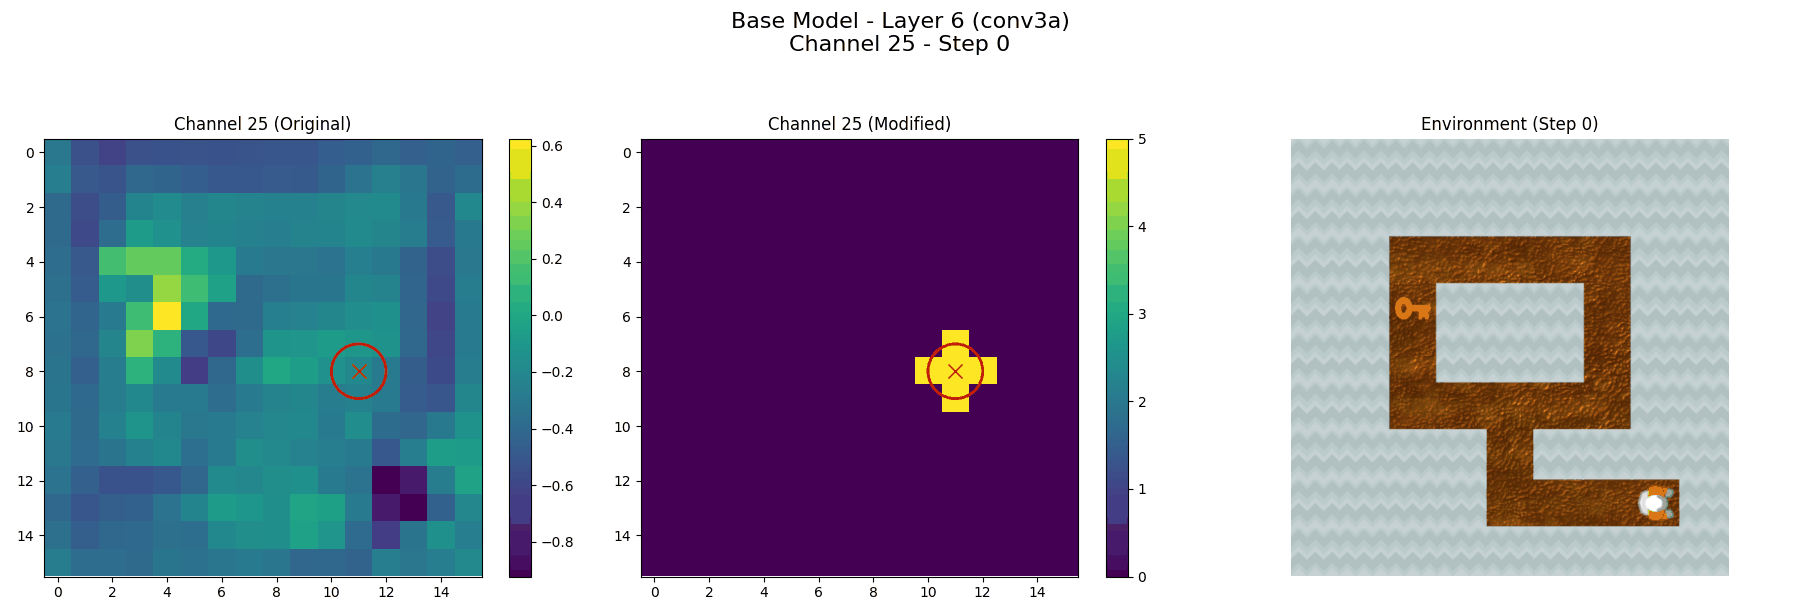
\includegraphics[width=1\textwidth]{figures/intervention_illustration.png}
    \caption{Example of the intervention experiment. We test channels to see the extent to which a single channel is capable of steering the agent to another location given the presence of a single entity in the environment. We consider an intervention a success if the agent enters the modified region. The maze is a 9 by 9 grid, while the conv4a channels have dimensions of 8 by 8, leading to a slightly imperfect mapping.}
    \label{fig:intervention-experiment}
    \end{figure}


    \subsection{Ablation Studies}
    \label{subsec:ablation_studies}
    To systematically assess the role of individual channels, a comprehensive ablation methodology was developed. For each channel in the SAE, episodes were run with only that channel active while ablating all other channels. This allowed measurement of the isolated capability of each channel to support navigation to different entities in the environment. Successful entity collection counts were recorded for each channel across multiple episodes.

    Because the agent has a bias towards randomly walking in a given direction depending on the current policy, it is necessary to rotate the maze so that the direction it's biased towards is the one facing away from the entities. This requires some manual intervention in order to ensure clarity in the results.


    \begin{figure}[h]
        \centering
        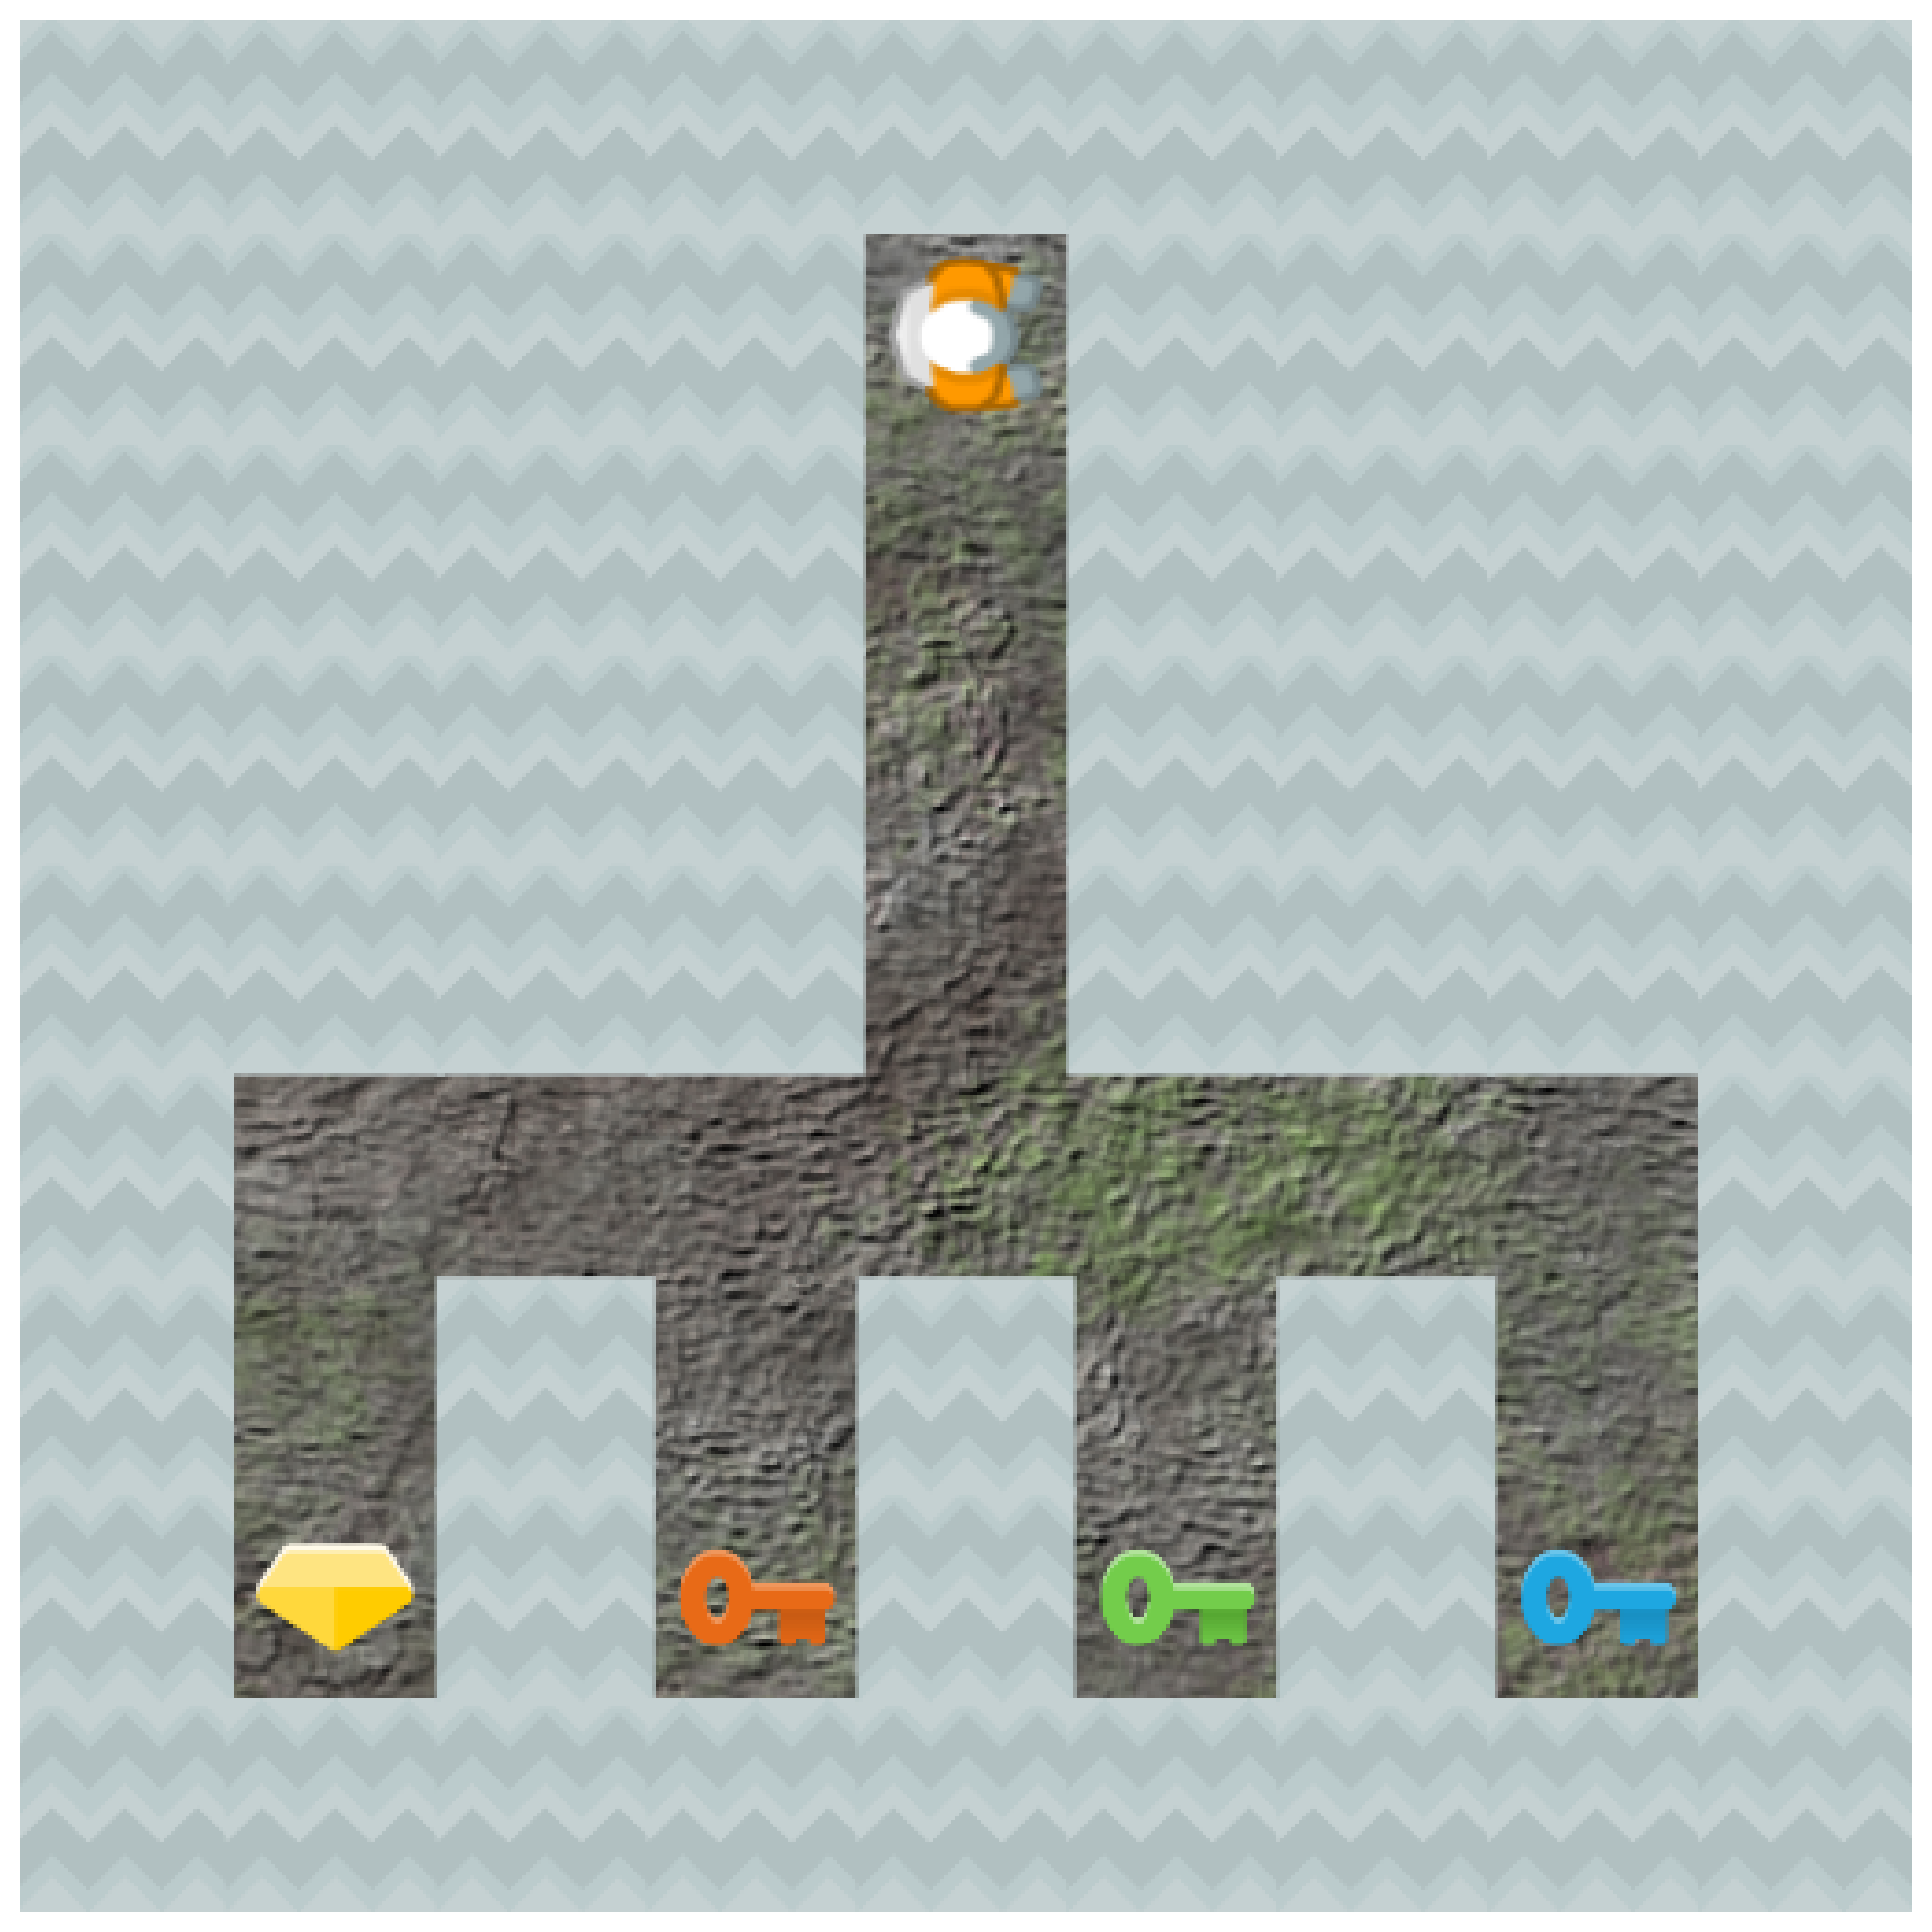
\includegraphics[width=0.8\textwidth]{figures/fork_maze_for_paper.png}
        \caption{The forked maze environment used for steering experiments. The agent starts at the top and must choose between navigating to the original entity (a key, in this case) on the left, or to the artificially targeted region on the right.}
        \label{fig:fork_maze_for_paper}
        \end{figure}

    \

\section{Experimental Design and Evaluation Metrics}


\label{sec:experimental_design_eval}
    \subsection{General Experimental Approach}
    \label{subsec:general_exp_approach}
    The research involved training RL agents and corresponding SAEs, followed by a series of analytical experiments. These experiments included feature visualization to understand learned representations, activation steering and patching to test causal control over agent behavior, and ablation studies to determine the functional importance of individual channels. The primary goal was to dissect how the agent represents and pursues multiple objectives in the Procgen Heist environment and how SAEs might alter or clarify these representations.

    \subsection{Evaluation Metrics}
    \label{subsec:eval_metrics}
    Several metrics were used to evaluate the different components of the research:
    \begin{itemize}
        \item \textbf{For SAE Training (Paper 1):} Performance was primarily tracked using variance explained (aiming for close to 1) and the reward attained on the maze-solving task after SAE integration (>95\% recovery). Sparsity was monitored by examining the number of dead features, the mean number of activating neurons, and the fraction of active neurons (target ~0.001).
        \item \textbf{For Steering and Activation Interventions (Paper 1 \& 2):} Success was measured by the agent's deviation to the artificially targeted zone or behavior change (e.g., moving away from an objective). For scaled-up experiments (Paper 1), the frequency of successful deviation across channels and activation strengths was recorded. For activation patching (Paper 2), the ability to steer the agent predictably was the primary metric.
        \item \textbf{For Ablation Studies (Paper 1):} The key metric was the count of successful entity collections per channel when all other channels were ablated, providing a quantitative measure of each channel's specialization and capability.
        \item \textbf{For Steering Vector Analysis (Paper 2):} The effectiveness of steering vectors was partly assessed by the steerability of different layers (reduction in objective pickups). Channel function was investigated by measuring the frequency with which a channel in an objective steering vector activated most strongly at the location of that particular objective.
    \end{itemize}

    \subsubsection{Intervention experiments}
    When doing our experiments, we would place a specific entity into the environment. We then intervene on a single channel in a single layer by applying a zero mask to the channel setting it to zero and setting a specific region of the channel to a chosen value. In this experiment, we would do a sweep over a range of intervention values between 0 and the maximum values that the channel would reach during typical functioning as determined by sampling from the environment during operation. By running this sweep, we can get a sense of what the different channels do at different intervention strengths. We kept the length of the episode to 20 steps to ensure that the agent would either be able to reach the target zone, or the actual entity, but not both.
    
    For each entity-channel combination, we ran 500 trials with the activation 
    value incrementing linearly: $v_i = i \cdot \frac{v_{\max}}{N}$, where $i$ 
    is the trial index (1 to $N$), $N=500$ is the total number of trials, and 
    $v_{\max}$ is the maximum activation range.
    
    We use a `Q' shaped maze with the design visible in\ref{fig:intervention-experiment} because it was challenging enough that the agent would need to retain its navigational abilities to reach either target, while providing a clear decision point where the agent would need to choose between pursuing the original entity or our artificial target zone. 
    
    We test a single entity at a time in this way meaning that steering that is effective with a particular value on a given channel may not be effective for redirecting the agent in the presence of another entity.
    
    To confirm that our results are robust, we also train SAEs~\cite{bricken2023monosemanticity} on the convolutional layers using techniques from~\cite{gorton_2024_missing} to confirm that the results are not merely the result of polysemanticity.

    \subsection{Channel Ablation Study}
To systematically assess the role of individual channels, we developed a comprehensive ablation methodology. For each channel in the network, we ran episodes with only that channel active while masking all other channels to zero. This allowed us to measure the isolated capability of each channel to support navigation to different entities in the environment. We recorded successful entity collection counts for each channel across  400 rollouts, providing a quantitative measure of each channel's specialization and capability. This methodology allows us identify which channels are sufficient for basic navigation. An example of the maze used is given in \ref{fig:ablation-mazes}.

\begin{figure}[H]
\centering
\begin{minipage}[b]{0.48\textwidth}
    \centering
    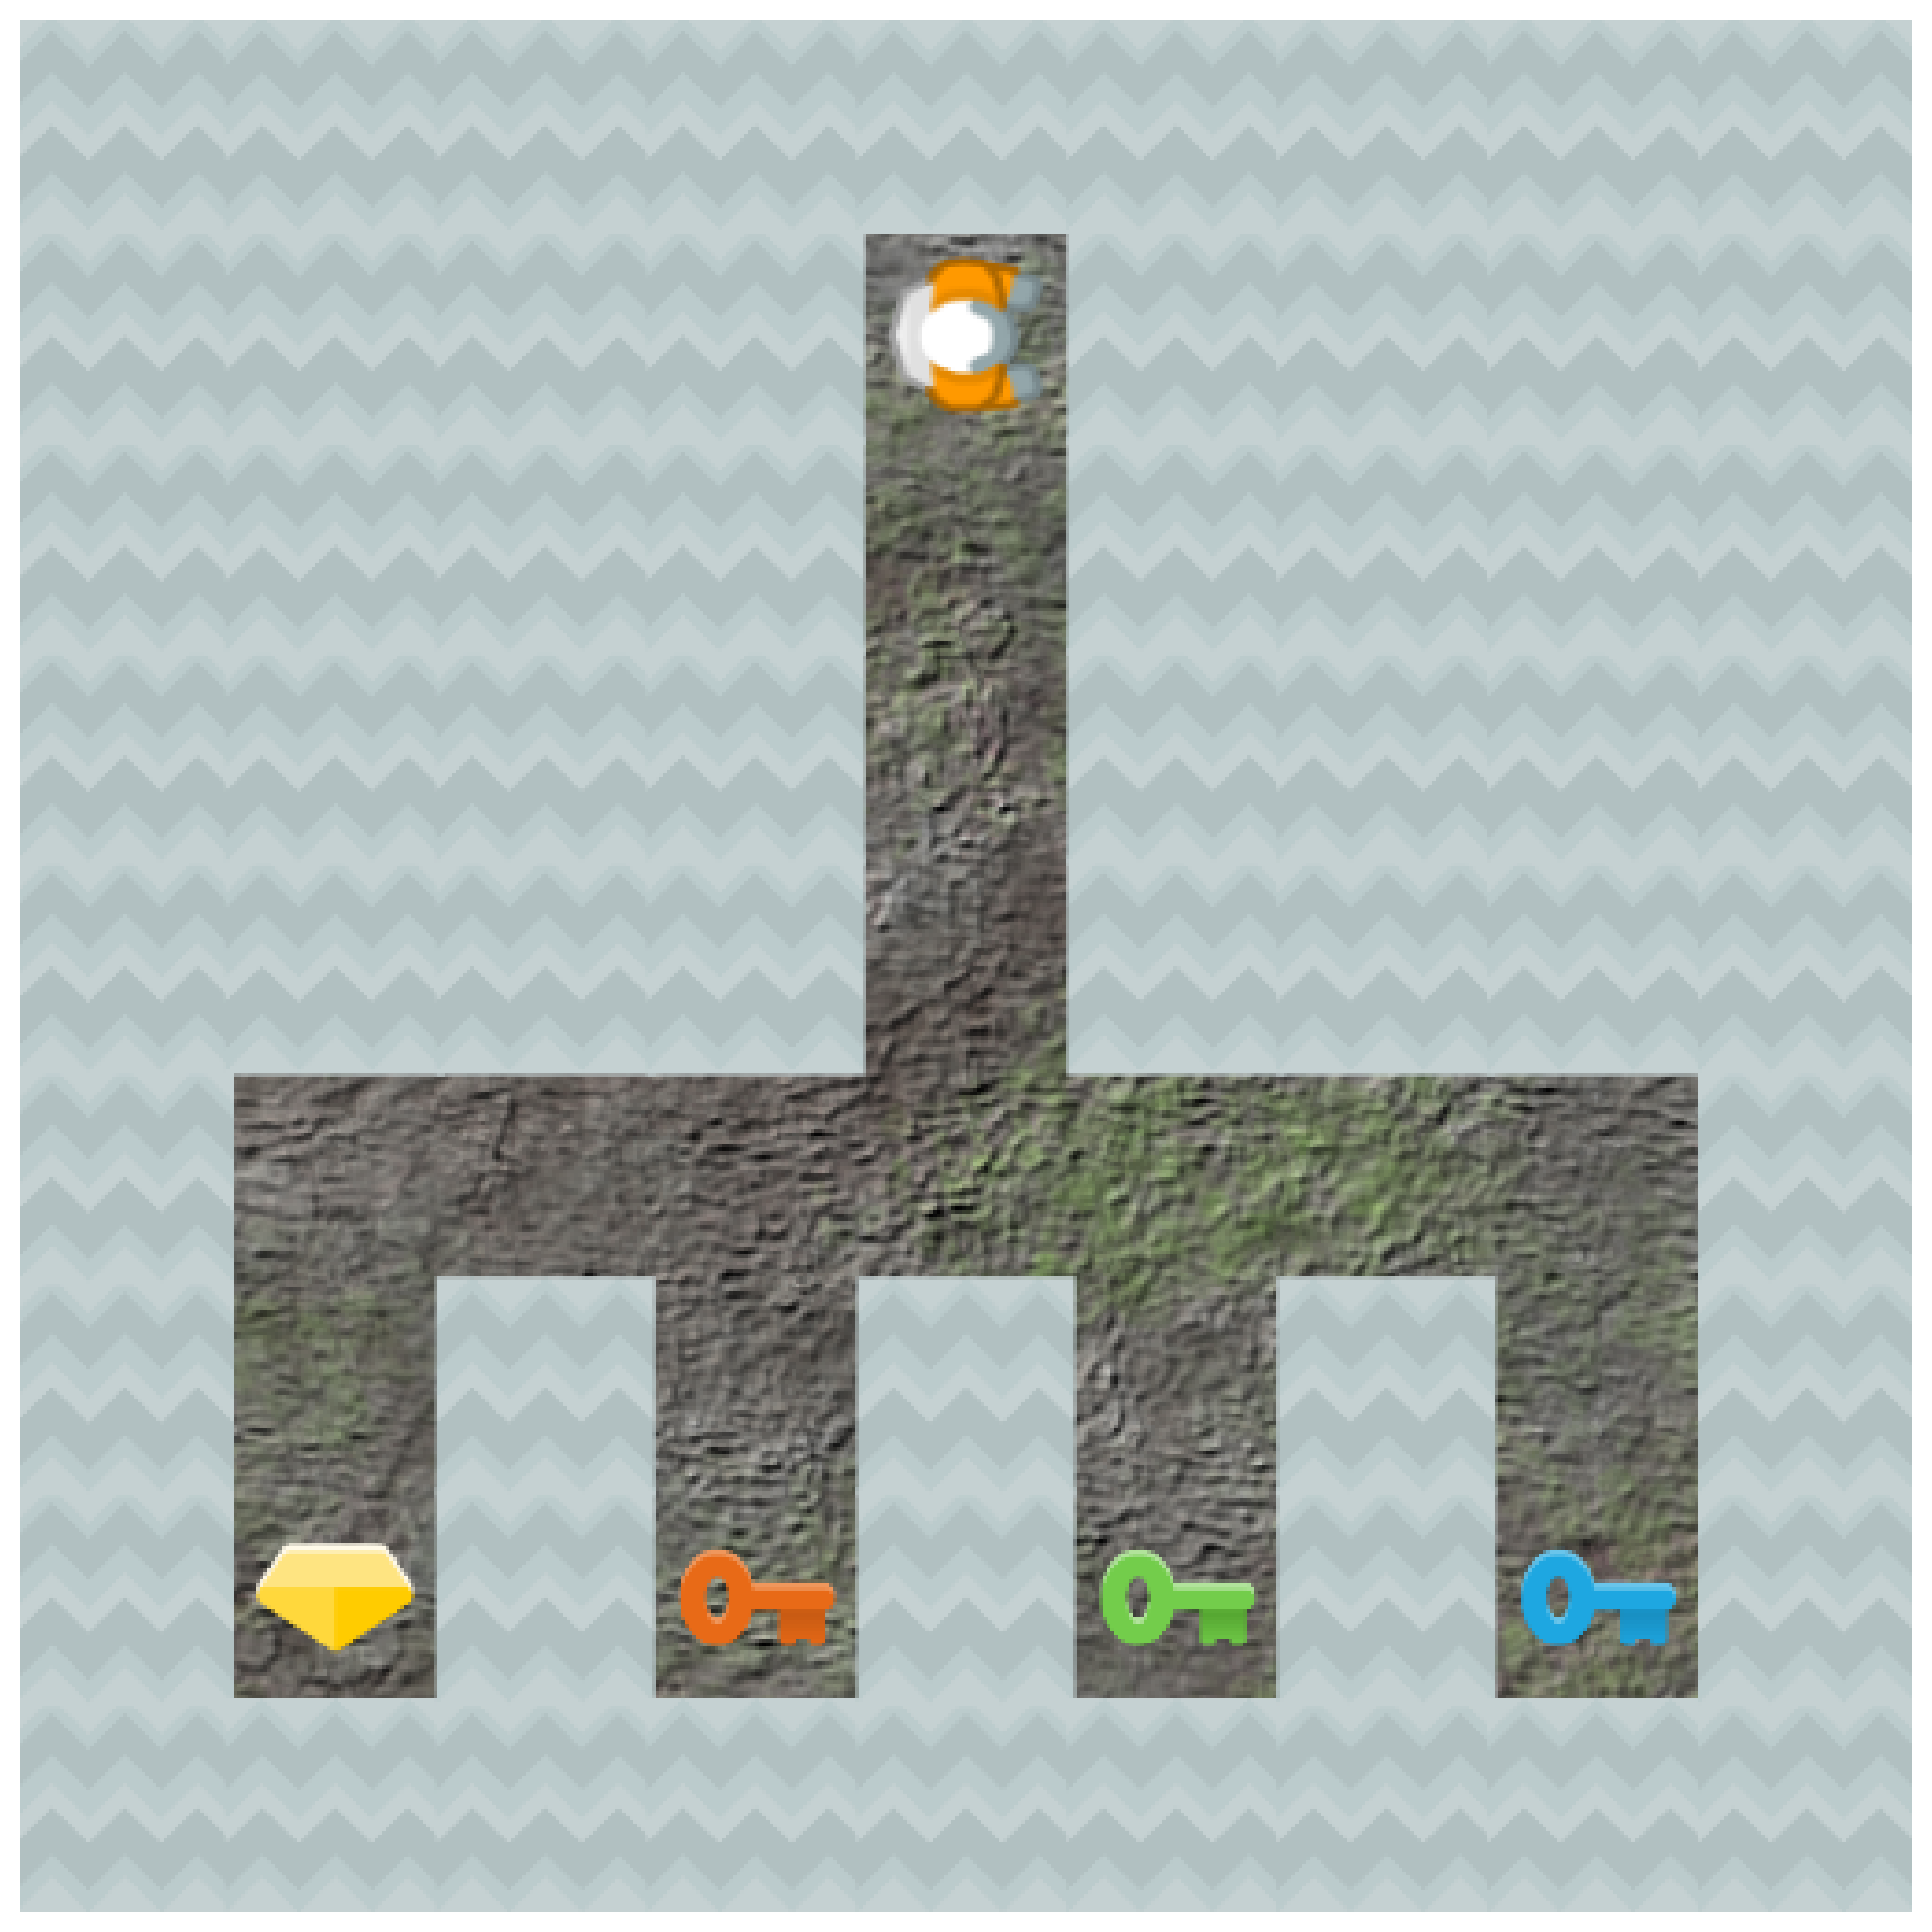
\includegraphics[width=\textwidth]{figures/fork_maze_for_paper.png}
\end{minipage}
\hfill
\begin{minipage}[b]{0.48\textwidth}
    \centering
    % TODO: Add empty_corners_maze_clean.png when available
    \includegraphics[width=\textwidth]{figures/empty_corners_maze_clean.png}
\end{minipage}
\caption{Maze configurations for ablation studies. (a) Fork maze tests individual channel navigation capability by requiring explicit path choices towards different entities and providing sufficient complexity that navigational abilities must be preserved. We orient the stem toward the model's inherent bias direction to minimize false positives. (b) Open maze with entities in corners tests the effect of ablating intervention spans without navigational constraints, ensuring only preferences regarding entity collection are observed.}
\label{fig:ablation-mazes}
\end{figure}
\subsection{Expanded ablation experiments}
To derive further insights from our earlier results, we ablate regions of the network based on their success in modifying model behavior in the previous experiments. Our experiment uses a modified maze which removes all walls, and has the keys and gem randomly distributed in the corners of the maze.

We perform four targeted ablations based on our steering and navigation findings:

\textbf{Ablation 1 (Intervention spans):} We zero out any activations within the value ranges that successfully steered the agent. Specifically, for entity $e$ and channel $c$, we set $h_{c,i,j} = 0$ whenever the activation falls within the successful steering range $\mathcal{S}_{e,c}$ identified in our intervention experiments.

\textbf{Ablation 2 (Navigation channels):} We completely ablate the top 10 channels identified as navigation-critical in our channel isolation study, setting these channels to zero while preserving all others.

\textbf{Ablation 3 (Combined):} We apply both ablations simultaneously, zeroing both the navigation channels and the intervention spans.

\textbf{Ablation 4 (Inverse):} We preserve only the intervention spans that successfully steered the agent in the presence of entity $e$, ablating everything else. This tests whether these spans alone are sufficient for navigation.

\section{Summary}
\label{sec:method_summary_revised}
This chapter detailed the methodologies employed to investigate goal representation and control in a deep reinforcement learning agent. It began with a description of the Procgen Heist environment and the model architectures used. Key interpretability techniques were then outlined, including the training of Sparse Autoencoders, feature visualization methods, the calculation and application of steering vectors for activation interventions, and systematic ablation studies. Finally, the experimental design and the quantitative and qualitative metrics used for evaluation were presented, providing a framework for understanding the results discussed in the subsequent chapter.

\chapter{Results}
\label{ch:results}

\section{Overview of Experiments}
\label{sec:exp_overview}
% Brief reminder of the experiments conducted
% Structure of the results presentation

\section{Performance of Reinforcement Learning Models}
\label{sec:rl_performance}
% Results related to the base RL models
% Training curves, convergence, final performance

\subsection{Baseline Performance}
\label{subsec:baseline}
% Standard metrics for your RL tasks
% Comparison with established benchmarks

\subsection{Stability and Reproducibility}
\label{subsec:stability}
% Variance across multiple runs
% Statistical significance of results

\section{Interpretability Results}
\label{sec:interp_results}
% Outcomes from applying your interpretability methods
% Visualization of explanations

\subsection{Feature Attribution Analysis}
\label{subsec:feature_attr}
% Results from attribution methods
% Important state features identified

\subsection{Decision Boundary Visualization}
\label{subsec:decision_boundary}
% Visualizations of policy decision boundaries
% Insights gained from these visualizations

\section{Comparative Analysis}
\label{sec:comparative}
% Comparison with existing interpretability methods
% Strengths and weaknesses of your approach

\section{Case Studies}
\label{sec:case_studies}
% Detailed analysis of specific examples
% Deep dive into interesting instances

\section{Summary of Findings}
\label{sec:findings_summary}
% Synthesis of all results
% Key takeaways from the experiments

\chapter{Discussion}
\label{ch:discussion}

\section{Interpretation of Results}
\label{sec:interpretation}

\subsection{Activation-Level Entity Encoding as Primary Discovery}
Our findings regarding how channels encode multiple entities at different activation strengths reveal a sophisticated information compression mechanism. Rather than requiring separate channels for each entity type, the model has learned to use activation magnitude as an additional dimension for encoding information. This discovery—visible in parallel rollout experiments showing consistent offsets between entity trajectories (correlation 0.931 in conv4a)—represents our most significant finding.

The ability to completely redirect agent behavior through uniform activation offsets (93\% blue key collection shifting to 94\% green key at +4.8 offset) demonstrates this encoding is causally central to network function. This suggests that interventions on neural networks need to consider not just which channels to modify, but also the precise activation values to use.

This activation-level encoding helps explain why the model can maintain full functionality with so few active channels—the network has effectively learned to multiplex information within individual channels. Due to the similarity of the task of tracking each key, it proves efficient to repurpose channels already capable of entity detection, having them target each entity sequentially while indicating the specific entity through activation strength.

\subsection{The Dead Channel Phenomenon in SAEs}
% From Paper 1 Discussion
The finding that a majority of steerable channels in the SAEs were `dead channels' (i.e., channels that exhibit no activation under normal circumstances) is a significant observation. This seemingly counterintuitive result has a clear mechanistic explanation rooted in the SAE architecture used (1x1 convolutional layers). In such an architecture, there is a direct one-to-one relationship between hidden channels in the SAE and their corresponding decoder weights. When a hidden channel dies (ceases to activate during normal forward passes), the gradient flow to its associated decoder weights stops. This effectively freezes those decoder weights at the values they had achieved before the channel became inactive.
Crucially, even though these channels do not activate during normal operation, their frozen decoder weights can still respond to artificial activation during intervention experiments. This explains why steering the agent is possible using channels that are otherwise silent – the learned patterns in their decoder weights are preserved and can be externally triggered. This implies that dead channels should not be automatically dismissed as unimportant in SAE analysis; they may preserve earlier learned representations that offer valuable insights into the model's learning trajectory and latent capabilities.

\subsection{Polysemanticity and Goal Representation in the Base Model}
% From Paper 2 Discussion
While prior work demonstrated interpretable channels in simpler environments (e.g.,\cite{mini_2023_understanding} in Procgen Maze), agents trained in more complex, multi-objective environments like Procgen Heist tend to develop highly polysemantic representations in their base networks. Most early-layer channels, and many in later convolutional layers, activate across multiple, diverse entities, making it challenging to assign singular, clear functional roles. Despite this polysemanticity, steering vectors proved to be a useful tool for isolating goal-related activity. Measuring the sparsity of these vectors allowed for the identification of channels in later layers that reliably track specific goals, even when these goals appear in varied spatial configurations.
These results suggest different layers of abstraction within the model: lower layers appear to capture general visual features and multiple entity types, while later layers consolidate this information into more actionable, goal-directed signals. The methods used offer a diagnostic approach to probing this transition and identifying functionally important parts of the network, even amidst widespread polysemanticity.

\subsection{Solution Multiplicity and Representational Drift}
A striking observation from our experiments was that intervention positions changed completely across different checkpoints even after convergence. Despite maintaining similar performance, the network continued exploring different encoding schemes within the solution space. This is largely due to the fact that we trained the model with an endless variety of maze variations rather than a fixed number, meaning it continued to adapt and change over time. This configuration was also the only one that led to successful training of our smaller model.

This variety of solutions suggests that amplitude-based multiplexing is not a unique solution but rather one of many equivalent representations the network can adopt, and a pattern which is likely to emerge over the course of training. The continuous drift between encoding schemes post-convergence indicates the network exists on a `valley floor' of equally viable solutions, constantly reorganizing its internal representations while preserving behavioral performance. 

We find a notable checkpoint at update step 30001 where no steerable channels at all are found for any entity, though we only found 1 example of this in the 60 checkpoints we tested, suggesting it might be less optimal than those with the stronger intervention configuration.

This has meaningful implications for approaching understanding the inner workings of models. The specific channels and activation ranges we identify for steering are not fixed properties of the task but rather snapshots of a dynamic system exploring equivalent representations as possible solutions. This representational drift may explain some of the difficulty in creating robust interpretability tools and suggests that interventions may need to be continuously recalibrated as networks evolve, though the extent to which this phenomena occurs beyond RL is unknown. 


\subsection{Activation-Level Entity Encoding}
Our findings regarding how the intervention spans encode multiple entities at different activation strengths reveal a sophisticated information compression mechanism. Rather than requiring separate channels for each entity type, the model has learned to use activation magnitude as an additional dimension for encoding information. This suggests that interventions on neural networks may need to consider not just which channels to modify, but also the precise activation values to use.

This activation-level encoding also helps explain why the model can maintain full functionality with so few active channels, the network has effectively learned to multiplex information within individual channels. 

An explanation for why this happens might be that due to the similarity of the task of tracking each key, it proves the most efficient solution to have re-purpose channels already capable of entity detection in general, and to have them simply target each one sequentially, while indicating the nature of the given entity by varying the activation strength.

\subsection{Role specialization}

A surprising finding was that some channels seem able to unilaterally alter where the agent will navigate to, many other channels were more reliably able to navigate the agent when the other channels were ablated, but were completely unable to individually steer the agent, as evidenced by examining \ref{fig:steering-dot-plot} and \ref{fig:ablation-heatmap}. This indicates that the specific function of indicating that the agent `must go to this spot' were exclusive to the steering channels, and the channels that were more successful in navigating had a role specifically in identifying how to get to a position, that in the absence of any other channels providing contrasting signals would lead the agent to go to that position. 

This idea of specialization and reliance between channels is reinforced by the fact that ablating both the navigation channels and the intervention spans produced better collection rates than ablating the best navigation channels while leaving the intervention spans untouched. The fact that this occurred 52\% of cases with n=400 trials is evidence that this effect is robust and not just noise.


\section{Theoretical Implications}
\label{sec:theoretical}
% How your results contribute to theory
% New insights about RL interpretability
The findings from this research contribute to the theoretical understanding of mechanistic interpretability in deep reinforcement learning in several ways. The demonstration of activation-level encoding suggests that neural networks may employ more nuanced information encoding strategies than simple feature presence/absence, utilizing the analog nature of activations as an additional information dimension. This challenges some simpler models of feature representation and highlights the potential for information multiplexing as a core principle of neural computation, especially when under pressure for representational efficiency.

The dead channel phenomenon in SAEs, and its mechanistic explanation, provides a concrete example of how network components that appear non-functional during standard inference can retain latent capabilities and learned knowledge. This has implications for how we assess model capacity and robustness, and for understanding the learning dynamics that lead to such states.

One observation from carrying out this work is that uncovering the role of activation magnitude across entire layers as a selection mechanism was difficult to uncover using typical mechanistic interpretability tools such as probes and SAEs. The most important discovery regarding how the network functioned (activation level entity encoding) turned out to be explicable purely by analysing the mean activations of different channels. It is possible that there may be further interesting discoveries to be made using similar approaches, particularly in networks that would likely benefit from recycling certain functionality for similar tasks that require clear delineation.

For RL interpretability specifically, this work underscores that techniques successful in one domain (e.g., LLMs) or simpler environments may need adaptation or re-evaluation in more complex, interactive settings. The interplay between learned environmental structure (like sequential objectives in Heist) and emergent network representations is a key area for future theoretical development.

\section{Practical Applications}\label{sec:applications}
% Real-world applications of your methods
% Potential use cases in different domains
While this research is primarily foundational, aiming to understand the internal workings of RL agents, the insights gained could have several long-term practical applications. A deeper understanding of how agents represent goals and make decisions can inform the development of more robust and reliable RL systems. For instance, identifying critical control channels or specific activation patterns linked to desired (or undesired) behaviors could lead to methods for:
\begin{itemize}
    \item \textbf{Enhanced Safety and Control:} Modifying or monitoring these identified neural correlates could provide mechanisms to prevent catastrophic failures or to guide agent behavior in critical situations.
    \item \textbf{Improved Debugging and Diagnostics:} When an RL agent fails or behaves unexpectedly, the ability to inspect specific features or channels (especially those disentangled by SAEs) could significantly speed up the debugging process.
    \item \textbf{More Sample-Efficient Learning:} Understanding what representations are crucial for a task might eventually lead to techniques that encourage or bootstrap the learning of these representations, potentially improving sample efficiency.
    \item \textbf{Agent Alignment:} Identifying how an agent represents complex or potentially conflicting goals is a step towards ensuring that agents behave in accordance with human intentions, a key challenge in AI alignment.
\end{itemize}
The techniques themselves, such as targeted activation steering or the analysis of SAE latents, could become part of a standard toolkit for RL practitioners seeking to verify and validate their models beyond simple performance metrics.

\section{Limitations of the Study}\label{sec:limitations}
% Honest assessment of limitations
% Factors that might affect validity or generalizability
This research, while providing several insights, is subject to certain limitations:
\begin{itemize}
    \item \textbf{Specificity to Architecture and Environment:} The findings are based on specific CNN architectures trained on the Procgen Heist environment. While efforts were made to use simplified, interpretable models and to validate on standard architectures (Paper 2), the extent to which these detailed mechanistic findings generalize to vastly different architectures (e.g., Transformers, RNNs) or other complex RL environments remains an open question.
    \item \textbf{Entangled Activations:} As noted in Paper 2, many goal-related activations in the base model remain entangled across channels. While SAEs aim to disentangle these, the disentanglement may not be perfect, and some interpretations might still be confounded by residual polysemanticity or distributed representations.
    \item \textbf{Off-Distribution Behavior:} Intervention experiments, by their nature, can push the network into off-distribution activation states. While this is useful for causal testing, the agent's behavior under such strong artificial interventions might not fully reflect its operational characteristics under normal, on-distribution conditions.
    \item \textbf{Incomplete Mapping of Channel Functions:} While specific channels and their roles were identified, a complete, precise map of all channels and their exact contributions to various sub-tasks or representations was not achieved. The complexity of the network, even simplified ones, makes such exhaustive mapping a significant challenge.
    \item \textbf{SAE Interpretation Nuances:} The interpretation of SAE latents themselves can be complex. It is not always clear if the features learned by an SAE perfectly mirror the computations of the base model or if they represent a re-factorization that is useful but distinct. The stability of SAE training and its impact on the consistency of learned features across different training runs or minor hyperparameter changes is also a consideration (Paper 1).
    \item \textbf{Focus on Convolutional Layers:} The primary focus of intervention and SAE application was on the convolutional layers. While these are crucial for visual processing and early planning, a full understanding would also require similar deep dives into the fully connected layers and the policy/value heads.
\end{itemize}

Our work is currently limited by the fact that we test only on a single environment, as there are not many environments that have similar qualities such as the extreme generalization encouraged by Procgen, and the sequential goals that Heist contains. To address this, future work could attempt this with MiniGrid environments, though a custom configuration that can establish similar diversity may be needed.

It is also unclear to what extent the intervention channel multiplexing phenomena generalises to other architectures, and we plan to test this in future work.

We also fail to provide an explanation of the specific mechanism played by the intervention channels. We plan to address this directly through a thorough application of probes that are trained to detect which entity is currently the next entity in order of pursuit by the network. Early work shows that the later convolutional layers do this very successfully, as well as the first fully connected layer. However, to truly understand the role of the intervention spans and navigation channels, it may be necessary to train probes on every channel and every row in the fully connected layer to determine their function. 

Our approach of simply intervening in every channel with 400 different activation strengths is also an approach that would need to be approached more carefully, due to cost constraints, in larger models. 

\section{Future Research Directions}\label{sec:future}
% Suggestions for further research
% Unsolved problems and next steps
The findings and limitations of this work point to several promising avenues for future research:

% From Paper 1 Future Work
\begin{itemize}
    \item \textbf{Tracking Non-Current Objectives:} Further exploration is needed into how RL agents internally represent and track entities or sub-goals that are not the immediate next target in a sequence, and whether interventions can reliably switch the agent's focus to these deferred objectives.
    \item \textbf{Application to Different Architectures:} Extending this line of inquiry to more complex agent architectures, such as decision transformers or RNN-style networks, would be valuable. These architectures have different mechanisms for handling temporal information and memory, and training probes or performing targeted interventions in their residual streams or hidden states could yield new insights.
    \item \textbf{Deeper Investigation of Activation Strength Encoding:} The phenomenon of activation strength encoding entity identity within SAE channels warrants further investigation. Understanding the precise mechanisms and robustness of this encoding could be highly beneficial.
    \item \textbf{Exploring Other Environment Entities:} This work focused primarily on keys and the gem. Future studies could investigate if other visual cues (e.g., the image of collected keys in a UI element) trigger steerable behaviors related to corresponding objectives (e.g., locks).
    \item \textbf{Advanced Attribution Techniques:} Applying more advanced techniques like attribution-based parameter decomposition~\citep{braun_2025_interpretability} to networks like the one studied here could yield valuable and potentially generalizable insights into how parameters contribute to function.
    \item \textbf{SAEs and Base Model Correspondence:} Investigating whether the functionalities highlighted or preserved by SAEs (such as entity encoding via activation strength) truly reflect similar underlying mechanisms in the base model, or are emergent properties of the SAE compression process, is a critical follow-up question.
\end{itemize}

% From Paper 2 Future Work / Discussion points framed as future work
\begin{itemize}
    \item \textbf{Robust Isolation of Goal-Related Circuits:} While steering vectors and SAEs help, further development of tools like causal tracing or more advanced sparse coding methods could be effective in more robustly isolating complete goal-related circuits, especially in the presence of significant polysemanticity.
    \item \textbf{Impact of Environment Design on Learned Representations:} Investigating how variations in environment design (e.g., training models with no fixed ordering of objectives in the maze) affect the development of generalizable circuits for goal pursuit would be an interesting direction.
    \item \textbf{Synthesizing Distributed Information:} Developing tools or models capable of synthesizing information from across different parts of the network is crucial, as the factors contributing to a specific outcome are often distributed. SAEs are one step in this direction, but further methods are needed.
\end{itemize}

\section{Reflections on the Research Process}\label{sec:reflections}
% Personal insights gained
% Challenges encountered and overcome
(This section is for your personal reflections on the research journey, challenges faced, and lessons learned. This content should be written by you.)

\chapter{Conclusion}\label{ch:conclusion}

\section{Summary of the Research}\label{sec:research_summary}

This work investigated how deep reinforcement learning agents internally represent and pursue sequential goals in the procedurally generated Procgen Heist environment. Using mechanistic interpretability techniques such as linear probes, activation interventions, parallel rollout analysis, and SAEs, we investigated the core mechanism behind how our network learned to encode goal structures in this multi-objective task and whether interpretability tools developed for language models translate to RL agents.

\section{Addressing Research Questions and Hypotheses}
\label{sec:addressing_rq}

Before interpreting our findings in detail, we first highlight the original research questions and hypotheses from Chapter~\ref{ch:introduction} and the extent to which they have been answered.

\subsection{Hypothesis Testing}

\begin{table}[h]
\centering
\caption[Hypothesis outcomes summary]{Hypothesis outcomes with key supporting evidence.}
\label{tab:hypothesis_outcomes}
\begin{tabular}{p{0.08\textwidth}p{0.35\textwidth}p{0.15\textwidth}p{0.45\textwidth}}
\toprule
\textbf{H\#} & \textbf{Hypothesis} & \textbf{Outcome} & \textbf{Key Evidence} \\
\midrule
H1 & Dedicated entity channels & \textbf{Partial} & Conv1a specialised, conv2-4a multiplex \\
H2 & SAEs disentangle features & \textbf{Rejected} & SAEs preserve multiplexing structure \\
H3 & Hierarchical preferences & \textbf{Confirmed} & 93\% blue key collection at baseline (cross maze)\\
H4 & SAEs successfully recover performance & \textbf{Confirmed} & 99.6-102\% recovery \\
H5 & Layer specialization & \textbf{Confirmed} & Entity $\rightarrow$ direction transition proven \\
\bottomrule
\end{tabular}
\end{table}

While some of our initial hypotheses proved correct, we were surprised by the discovery of the spatial gating mechanism, where negative activations mark regions of interest and shift systematically as objectives are completed. We also found that SAEs did not work as expected in this case, but as a result were able to validate some of our new results. We were also able to better characterise some of our initial ideas about how the network might work.

\subsection{Research Questions}

\begin{table}[h]
\centering
\caption[Research questions and answers]{Research questions and their answers based on experimental evidence.}
\label{tab:rq_outcomes}
\renewcommand{\arraystretch}{1.5} % Adds 50% more vertical space
\begin{tabular}{p{0.08\textwidth}p{0.35\textwidth}p{0.55\textwidth}}
\toprule
\textbf{RQ} & \textbf{Question} & \textbf{Answer} \\
\midrule
RQ1 & How are goals encoded? & Via spatial gating where negative activations mark regions of interest (Section~\ref{sec:parallel_rollouts},~\ref{sec:negative_activations}) \\
RQ2 & How is the current target determined? & Two-phase: detection at conv1a $\rightarrow$  integration at conv2a-conv4a (Table~\ref{tab:probe_whole_layer}) \\
RQ3 & Can SAEs clarify feature roles? & Yes, but only providing validation (Section~\ref{subsec:sae_structure}) \\
RQ4 & Dedicated vs general channels? & Conv1a specialised conv2a-conv4a generalised (Appendix~\ref{app:channel_probe_results}) \\
RQ5 & Why different steering success rates across entities? & Gem spans in 31/32 channels vs 14 for keys may explain differential steering (Table~\ref{tab:ablation_results}) \\
RQ6 & Do layers have specialised roles? & Yes: entity detection in conv layer, navigation in fc2 (Tables~\ref{tab:probe_whole_layer},~\ref{tab:probe_directional}) \\
\bottomrule
\end{tabular}
\end{table}

\section{Key Findings and Contributions}
\label{sec:contributions}

We primarily demonstrate the unusual and previously undocumented phenomenon of the network using spatial gating to track game state, where negative activations mark regions of interest and shift systematically as objectives are completed. We show this through the clear parallel trajectories of activations as demonstrated by the parallel rollout experiments that have an extremely high correlation (r=0.931 in conv4a), demonstrating that the same channels are active across different game states but at systematically different levels. Most surprisingly, we are able to achieve clear and consistent shifts in behaviour that maintain core network functions with only a simple constant offset to all channel weights, likely by mimicking the activation patterns characteristic of different game stages. This highlights a significant gap in current approaches to MI research, which focuses on identifying which parts of the network are responsible for a certain activation, but fails to consider how temporal patterns in activation levels may encode task progress. 

We further identified a bimodal structure in the network regarding target entity identification early in the network, and a surge in correctly identifying the correct direction to travel later in the network. Entity information crystallizes to 99.3\% probe accuracy in conv3a before collapsing to 20.4\% in fc3, while directional information is not as strong in early layers but strengthens to 67.3\% in fc2. This reveals that convolutional layers determine where things are in the maze before the FC layers determine how to arrive there. This explains why our interventions in the convolutional layers are able to succeed before targets have crystallized.

We also found that SAEs, while of some use in validating our results, failed to provide a great deal of additional insight into the network that would not have been gained otherwise. This highlights the potential pitfalls of trying to apply promising tools before considering simple interventions and experiments that may lead to more insight.

\section{Limitations of the Study}\label{sec:limitations}

This research, while providing several insights, is subject to certain limitations:

Our work is currently limited by the fact that we test only on a single environment, as there are not many environments that have similar qualities such as the extreme generalization encouraged by Procgen, and the staged multi-goal configuration in Heist. To address this, future work could attempt this with MiniGrid environments, though a custom configuration that can establish similar diversity may be needed.

It is also unclear to what extent the intervention channel multiplexing phenomenon generalises to other architectures, and we plan to test this in future work.

Our training methodology differs from standard practice in using unlimited procedurally generated environments rather than the typical 200-500 set of environments one would set. While this was necessary for successful training with our compressed architecture, it may affect the generalization of our findings to models trained under standard Procgen protocols. The unlimited environment diversity likely also contributes to the representational drift we observe, as the network continually trains on new environmental distributions.

We also do not yet fully characterise the function of the intervention spans, or if they translate to an actual unique role within the network's natural functioning. We plan to address this directly through a thorough application of probes that are trained to detect which entity is currently the next entity in order of pursuit by the network. Early work shows that the later convolutional layers do this very successfully, as well as the first fully connected layer. However, to truly understand the role of the intervention spans and navigation channels, it may be necessary to train probes on every channel and every row in the fully connected layer to determine their function.

Intervention experiments, by their nature, can push the network into off-distribution activation states. While this is useful for causal testing, the agent's behaviour under such strong artificial interventions do not represent its typical behaviour. We do not yet have a clear picture of precise circuitry under normal operating conditions. Additionally, the patching interventions were typically only applied with positive activations, but the mean channel activation analysis shown in Figure~\ref{fig:activation_tracking} reveals that for many channels the activations of the network are mostly negative. This means that a large portion of their activity is not being captured accurately in the interventions. We believe future work in understanding the role of the negative activations in the convolutional channels would lead to fruitful insights.

Our approach of simply intervening in every channel with 400 different activation strengths is also an approach that would need to be approached more carefully, due to cost constraints, in larger models.

\section{Future Work}\label{sec:future_work}

This research opens several promising avenues for future investigation. The discovery of spatial gating through activation polarity suggests examining whether similar mechanisms exist in other architectures and domains, particularly in transformer-based models where activation patterns might track different modes of operation.

Testing this mechanism across different RL environments, especially those with hierarchical goal structures or mode-switching requirements, could reveal whether spatial gating is a general principle of efficient neural computation under resource constraints.

The methodological insight that simple mean activation analysis revealed what sophisticated tools missed suggests revisiting other `well-understood' models with basic statistical approaches. This could uncover overlooked organizational principles, particularly in systems previously deemed too polysemantic for interpretation.

The precise control achievable through small activation offsets ($\pm$0.5 at conv2a) warrants investigation into whether training procedures could be designed to encourage such structures, potentially yielding models that are interpretable and controllable by design rather than post-hoc analysis.

Finally, the two-phase architecture's clear separation between `what to target' and `how to navigate' suggests applications in hybrid systems where interpretable goal selection could be combined with powerful but opaque execution modules, potentially offering a path toward more trustworthy autonomous systems.

\section{Final Remarks}
\label{sec:final_remarks}

This thesis demonstrates the practicality of understanding such neural networks, though it also highlights some key bottlenecks in doing this at scale. In particular, many of the tools that have been developed to interpret such models were not able to capture key parts of the network's functioning. This highlights that there are still significant gaps in the way that we approach thinking about neural networks, and in particular networks trained with RL. It also highlights the importance of examining fundamental structures such as activation patterns and high level statistics as a simple first step in approaching such problems.

Given the potential for activation-level encoding to extend beyond this specific environment and architecture, we hope that understanding this particular toy model may alter the way the reader thinks about neural networks, and that cracking the problem of the inner workings of such models may be easier as a result. 


% Bibliography
\printbibliography

\appendix
\chapter{Appendix Title}


\appendix
\section{Technical Appendices}

\appendix
\section{Model Architecture Details}
\label{app:model_architecture}


ImpalaCNN architecture:
\begin{figure}[H]
\centering
    \includegraphics[width=0.98\textwidth]{figures/diagram (2).pdf}
\caption{The convolutional neural network architecture used in our experiments. We use a modified version of the Impala CNN with 5 convolutional layers rather than the original 15 layers, which provides better interpretability without compromising performance.}
\label{fig:network-architecture}
\end{figure}
% Your appendix content goes here



\section{Activation offset results}
\label{app:additional_offset_results}


\begin{figure}[H]
    \centering
        \includegraphics[width=0.98\textwidth]{figures/offset_sweep_conv3a_expanded_checkpoint_35001_full_range.pdf}
    \caption{Full range activation offset sweep for conv3a layer at checkpoint 35001. Each subplot shows entity collection success rates across different activation offset values for a specific channel. This wide-range sweep reveals the broad activation ranges over which different channels can successfully steer the agent toward specific entities.}
    \label{fig:offset_steering_conv3a_full}
    \end{figure}

    \begin{figure}[H]
        \centering
            \includegraphics[width=0.98\textwidth]{figures/offset_sweep_conv3a_expanded_checkpoint_35001_-3to3_step0.03.pdf}
        \caption{Narrow range activation offset sweep for conv3a layer at checkpoint 35001, focusing on offset values from -3 to +3 with step size 0.03. This fine-grained sweep provides higher resolution detail of entity collection rates in the critical activation range where steering behavior transitions occur.}
        \label{fig:offset_steering_conv3a-3+3}
        \end{figure}
\begin{figure}[H]
\centering
    \includegraphics[width=0.98\textwidth]{figures/offset_sweep_conv2a_expanded_checkpoint_35001_-15to15_step0.1.pdf}
\caption{Wide range activation offset sweep for conv2a layer at checkpoint 35001, testing offset values from -15 to +15 with step size 0.1. This broader sweep examines the extent to which earlier convolutional layers can be steered across a wide range of activation offsets.}
\label{fig:offset_steering_conv2a-15+15}
\end{figure}

\begin{figure}[H]
    \centering
        \includegraphics[width=0.98\textwidth]{figures/offset_sweep_conv2a_expanded_checkpoint_35001_-1to1_step0.01.pdf}
    \caption{Narrow range activation offset sweep for conv2a layer at checkpoint 35001, focusing on offset values from -1 to +1 with step size 0.01. This high-resolution sweep examines fine-grained steering behavior in the conv2a layer's most sensitive activation range.}
    \label{fig:offset_steering_conv2a-1+1}
    \end{figure}

\begin{figure}[H]
    \centering
        \includegraphics[width=0.98\textwidth]{figures/offset_sweep_conv1a_expanded_checkpoint_35001_-3to3_step0.03.pdf}
    \caption{Activation offset sweep for conv1a layer at checkpoint 35001, testing offset values from -3 to +3 with step size 0.03. This sweep examines steering capabilities in the earliest convolutional layer, which operates closest to the raw input observations.}
    \label{fig:offset_steering_conv1a-3+3}
    \end{figure}

\section{Mean Activation Per Channel During Rollout}
\label{app:rollout_activation_analysis}

\begin{figure}[H]
    \centering
        \includegraphics[width=0.98\textwidth]{figures/standard_all_channels_35k_no_locks.pdf}
    \caption{Figure showing the mean activation per channel across all channels in the same rollout as presented in Figure~\ref{fig:activation_tracking}. We see that the pattern of increasing activation strength over the course of an episode with sharp jumps at the collection of different entities is shared across many but not all channels, with a few showing very consistent activation strengths from beginning to end. In general mean activations remain below 0 for all channels, indicating that a great deal of the neurons across channels are negative a majority of the time. }
    \label{fig:activation_rollout_all_channels}
\end{figure}


\begin{figure}[H]
    \centering
        \includegraphics[width=0.98\textwidth]{figures/simple_cross_maze_35k_no_locks_rollout_green_first_seed13.pdf}
    \caption{ Plot showing the mean activation values captured across all timesteps in an unmodified rollout in the 6 channels that had the greatest variance over the course of the rollout. The shaded regions indicate the current `next target', the entity that it would logically pursue next in solving the maze. In this rollout in the cross maze environment, the agent targeted the green key first. A similar uptick in positive values can be observed at the moment of green key collection, though the larger uptick in mean activations typically associated with the blue key can be observed at the moment of blue key collection as well.}
    \label{fig:activation_rollout_green_first}
\end{figure}

\section{Channel-Level Probe Results}
\label{app:channel_probe_results}

This section presents detailed per-channel probe accuracies for multi-class entity classification across convolutional layers. All probes were trained using logistic regression on individual channel activations to predict the next entity the agent will navigate toward (7-way classification: blue key, green key, red key, blue lock, green lock, red lock, gem). Lock entities are omitted from these tables for brevity, though they were included in the overall accuracy calculations. Random baseline performance is 14.3\%.

\subsection{Conv1a Layer - All Channels}

Table~\ref{tab:conv1a_channels} shows probe results for all 16 channels in the Conv1a layer. This layer exhibits the highest variance in channel performance, with the best channel (Ch0) achieving 97.1\% overall accuracy while the worst (Ch5) achieves only 14.7\%. Three channels (Ch0, Ch11, Ch12) demonstrate strong generalist performance across all entity types, suggesting they encode rich multi-entity representations.

\begin{table}[H]
\centering
\caption{Conv1a layer per-channel probe accuracies. All 16 channels shown. Bold indicates highest accuracy in each column.}
\label{tab:conv1a_channels}
\begin{tabular}{ccccccc}
\toprule
Channel & Overall & Blue Key & Green Key & Red Key & Gem \\
\midrule
0 & \textbf{97.1\%} & 97.7\% & 94.8\% & 98.1\% & \textbf{97.3\%} \\
1 & 17.7\% & 0.0\% & 0.0\% & 79.3\% & 45.1\% \\
2 & 65.1\% & 90.7\% & 14.5\% & 94.7\% & 90.2\% \\
3 & 20.3\% & 0.0\% & 3.5\% & 0.0\% & 50.5\% \\
4 & 17.2\% & 98.1\% & 0.0\% & 0.0\% & 4.4\% \\
5 & 14.7\% & 0.0\% & 0.0\% & 0.0\% & 0.0\% \\
6 & 21.9\% & 28.4\% & 0.0\% & 54.8\% & 0.0\% \\
7 & 16.1\% & 0.0\% & 0.0\% & 94.7\% & 0.0\% \\
8 & 21.1\% & 0.0\% & 61.6\% & 0.0\% & 53.8\% \\
9 & 14.9\% & 0.0\% & 0.0\% & \textbf{100.0\%} & 0.0\% \\
10 & 17.1\% & 0.0\% & 43.6\% & 76.0\% & 0.0\% \\
11 & 94.7\% & \textbf{100.0\%} & \textbf{98.3\%} & 90.4\% & 88.6\% \\
12 & 91.6\% & 99.5\% & 94.8\% & 88.5\% & 89.7\% \\
13 & 20.3\% & 0.0\% & 0.0\% & 54.3\% & 0.0\% \\
14 & 15.2\% & 2.3\% & 0.0\% & \textbf{100.0\%} & 0.0\% \\
15 & 17.7\% & 0.0\% & 0.0\% & 0.0\% & 48.4\% \\
\bottomrule
\end{tabular}
\end{table}

\subsection{Conv2a Layer - Top 10 Channels}

Table~\ref{tab:conv2a_top10} presents the top 10 performing channels in Conv2a (out of 32 total). This layer shows dramatically improved performance compared to Conv1a, with the best channel (Ch4) achieving near-perfect 99.4\% accuracy. The top channel achieves perfect accuracy on three entity types (blue lock, green lock, red lock, gem), suggesting highly disentangled representations.

\begin{table}[H]
\centering
\caption{Conv2a layer top 10 channels by overall accuracy (out of 32 total channels). Bold indicates highest accuracy in each column.}
\label{tab:conv2a_top10}
\begin{tabular}{ccccccc}
\toprule
Channel & Overall & Blue Key & Green Key & Red Key & Gem \\
\midrule
4 & \textbf{99.4\%} & 98.1\% & 98.8\% & \textbf{99.0\%} & \textbf{100.0\%} \\
27 & 98.9\% & 98.6\% & \textbf{99.4\%} & 96.6\% & \textbf{100.0\%} \\
1 & 95.2\% & 98.6\% & 96.5\% & 94.2\% & 98.9\% \\
25 & 93.9\% & 97.2\% & 94.8\% & 88.0\% & 96.2\% \\
14 & 90.4\% & 88.8\% & 94.2\% & 83.2\% & \textbf{100.0\%} \\
31 & 90.2\% & 92.6\% & 88.4\% & 86.1\% & 95.1\% \\
5 & 88.4\% & 92.1\% & 86.1\% & 75.0\% & 96.7\% \\
29 & 87.6\% & 95.4\% & 89.5\% & 77.9\% & 96.2\% \\
18 & 86.4\% & 88.4\% & 84.3\% & 77.4\% & \textbf{100.0\%} \\
16 & 85.5\% & \textbf{95.8\%} & 77.9\% & 70.7\% & 91.9\% \\
\bottomrule
\end{tabular}
\end{table}

\subsection{Conv3a Layer - Top 10 Channels}

Table~\ref{tab:conv3a_top10} shows the top 10 channels in Conv3a (out of 32 total). Interestingly, this layer shows lower per-channel performance than Conv2a (best: 82.9\% vs 99.4\%), despite whole-layer probes achieving 99.3\% accuracy. This suggests Conv3a relies more heavily on distributed representations across multiple channels rather than individual specialist channels.

\begin{table}[H]
\centering
\caption{Conv3a layer top 10 channels by overall accuracy (out of 32 total channels). Bold indicates highest accuracy in each column.}
\label{tab:conv3a_top10}
\begin{tabular}{ccccccc}
\toprule
Channel & Overall & Blue Key & Green Key & Red Key & Gem \\
\midrule
19 & \textbf{82.9\%} & \textbf{89.8\%} & \textbf{79.1\%} & \textbf{80.8\%} & 90.2\% \\
20 & 82.7\% & 77.2\% & \textbf{79.1\%} & 80.3\% & 88.6\% \\
9 & 78.6\% & 77.7\% & \textbf{79.1\%} & 76.4\% & 90.2\% \\
4 & 78.4\% & 83.7\% & 75.0\% & 72.1\% & 83.7\% \\
6 & 76.4\% & 84.7\% & 72.1\% & 73.1\% & 85.3\% \\
25 & 76.2\% & 79.1\% & 72.1\% & 62.5\% & \textbf{97.8\%} \\
23 & 75.6\% & 87.9\% & 66.9\% & 71.2\% & 85.3\% \\
2 & 74.4\% & 77.7\% & 66.3\% & 74.0\% & 86.4\% \\
3 & 74.1\% & 72.1\% & 69.2\% & 70.2\% & 89.7\% \\
21 & 73.9\% & 79.5\% & 61.6\% & 70.7\% & 87.5\% \\
\bottomrule
\end{tabular}
\end{table}

\subsection{Conv4a Layer - Top 10 Channels}

Table~\ref{tab:conv4a_top10} presents the top 10 channels in Conv4a (out of 32 total). This is the final convolutional layer before the fully connected layers. Notably, even the best channel (Ch18, 68.1\%) shows substantially lower performance than individual channels in earlier layers, despite whole-layer probes achieving 97.6\% accuracy. This indicates that Conv4a representations are highly distributed and no single channel carries sufficient information for accurate classification.

\begin{table}[H]
\centering
\caption{Conv4a layer top 10 channels by overall accuracy (out of 32 total channels). Bold indicates highest accuracy in each column.}
\label{tab:conv4a_top10}
\begin{tabular}{ccccccc}
\toprule
Channel & Overall & Blue Key & Green Key & Red Key & Gem \\
\midrule
18 & \textbf{68.1\%} & 83.3\% & 45.4\% & \textbf{70.7\%} & \textbf{88.0\%} \\
8 & 67.1\% & \textbf{86.5\%} & 50.0\% & 59.1\% & 73.4\% \\
17 & 64.9\% & 83.3\% & 55.2\% & 57.7\% & 78.3\% \\
28 & 63.0\% & 82.3\% & 51.2\% & 52.4\% & 79.9\% \\
10 & 62.0\% & 68.8\% & 55.2\% & 58.2\% & 78.8\% \\
0 & 61.9\% & 78.6\% & \textbf{56.4\%} & 55.3\% & 66.3\% \\
21 & 61.9\% & 71.2\% & 44.8\% & 61.5\% & 69.0\% \\
4 & 61.8\% & 74.4\% & 47.1\% & 52.4\% & 81.5\% \\
26 & 60.4\% & 74.0\% & 39.5\% & 51.4\% & 69.0\% \\
16 & 59.4\% & 82.3\% & 45.4\% & 56.3\% & 64.7\% \\
\bottomrule
\end{tabular}
\end{table}

\subsection{Summary of Channel-Level Findings}

Several patterns emerge from the channel-level probe analysis:

\begin{enumerate}
\item \textbf{Layer hierarchy}: Conv1a contains a small number of highly informative generalist channels (Ch0, Ch11, Ch12) alongside many specialist channels that encode only specific entities. Conv2a shows improved overall performance with multiple high-performing generalist channels. Conv3a and Conv4a show increasingly distributed representations where individual channels carry less information. 

\item \textbf{Distributed vs sparse coding}: The gap between whole-layer and best single-channel performance grows substantially in deeper layers (Conv3a: 99.3\% whole vs 82.9\% best channel; Conv4a: 97.6\% whole vs 68.1\% best channel), indicating a shift from sparse coding in early layers to distributed coding in later layers.

\item \textbf{Entity-specific patterns}: Some channels in Conv1a show extreme specialization (e.g., Ch9 and Ch14 achieve 100\% on red key but near 0\% on other entities), while Conv2a channels tend toward more balanced multi-entity performance.
\end{enumerate}


\section{Intervention spans across checkpoints}
\label{app:evolution_of_interventions}

Figures \ref{fig:intervention_40k}--\ref{fig:intervention_60k} illustrate the representational drift observed across checkpoints 40k-60k. Despite stable task performance, the specific channels exhibiting steering behavior and their associated activation ranges shift dramatically between checkpoints, demonstrating that the network continuously explores equivalent solutions within a broad basin of the loss landscape.

\begin{figure}[p]
\centering
\includegraphics[width=0.95\textwidth]{figures/entity_distribution_plot_focused_blue_key_gem_green_key_red_key_layer_conv4a_top_7_ood_p99.9_step_40001.pdf}
\caption{Steering intervention success rates for conv4a layer at checkpoint 40k. Colored dots represent successful steering interventions for different entities (blue key, green key, red key, gem), while black lines indicate the 99.9th percentile of normal activations. Each panel shows a different channel exhibiting steering behavior.}
\label{fig:intervention_40k}
\end{figure}

\begin{figure}[p]
\centering
\includegraphics[width=0.95\textwidth]{figures/entity_distribution_plot_focused_blue_key_gem_green_key_red_key_layer_conv4a_top_11_ood_p99.9_step_45001.pdf}
\caption{Steering intervention success rates for conv4a layer at checkpoint 45k. Colored dots represent successful steering interventions for different entities (blue key, green key, red key, gem), while black lines indicate the 99.9th percentile of normal activations. Each panel shows a different channel exhibiting steering behavior.}
\label{fig:intervention_45k}
\end{figure}

\begin{figure}[p]
\centering
\includegraphics[width=0.95\textwidth]{figures/entity_distribution_plot_focused_blue_key_gem_green_key_red_key_layer_conv4a_top_21_ood_p99.9_step_50001.pdf}
\caption{Steering intervention success rates for conv4a layer at checkpoint 50k. Colored dots represent successful steering interventions for different entities (blue key, green key, red key, gem), while black lines indicate the 99.9th percentile of normal activations. Each panel shows a different channel exhibiting steering behavior.}
\label{fig:intervention_50k}
\end{figure}

\begin{figure}[p]
\centering
\includegraphics[width=0.95\textwidth]{figures/entity_distribution_plot_focused_blue_key_gem_green_key_red_key_layer_conv4a_top_29_ood_p99.9_step_55001.pdf}
\caption{Steering intervention success rates for conv4a layer at checkpoint 55k. Colored dots represent successful steering interventions for different entities (blue key, green key, red key, gem), while black lines indicate the 99.9th percentile of normal activations. Each panel shows a different channel exhibiting steering behavior.}
\label{fig:intervention_55k}
\end{figure}

\begin{figure}[p]
\centering
\includegraphics[width=0.95\textwidth]{figures/entity_distribution_plot_focused_blue_key_gem_green_key_red_key_layer_conv4a_top_11_ood_p99.9_step_60001.pdf}
\caption{Steering intervention success rates for conv4a layer at checkpoint 60k. Colored dots represent successful steering interventions for different entities (blue key, green key, red key, gem), while black lines indicate the 99.9th percentile of normal activations. Each panel shows a different channel exhibiting steering behavior.}
\label{fig:intervention_60k}
\end{figure}

\section{SAE Intervention Results}
\label{app:sae_interventions}

The following figures show steering intervention success rates for SAE latents both trained on the 35000 step checkpoint. Unlike the base model channels (which have 32 dimensions per layer), the SAE uses a 4x expansion factor, resulting in 128 latents per layer. These figures demonstrate that sparse autoencoder latents can also be successfully steered to influence agent behavior toward specific entities. Colored dots represent successful steering interventions for different entities (blue key, green key, red key, gem), while black lines indicate the 99.9th percentile of normal activations during standard gameplay. Figures shown have a threshold for inclusion of $\geq 200$ successes for readability.

\begin{figure}[H]
\centering
\includegraphics[width=0.95\textwidth]{figures/entity_distribution_plot_focused_blue_key_gem_green_key_red_key_layer_conv3a_top_41_ood_p99.9.pdf}
\caption{SAE latent steering intervention success rates for conv3a layer, showing the top 41 most successful latents with a cutoff threshold of $\geq 200$ successes. Of particular note is the large number of steering successes in general in conv3a and also the significant overlap between different sections, including within similar activation regions, displaying relatively less of the multiplexing phenomena relative to elsewhere.}
\label{fig:sae_intervention_conv3a_41}
\end{figure}

\begin{figure}[H]
\centering
\includegraphics[width=0.95\textwidth]{figures/entity_distribution_plot_focused_blue_key_gem_green_key_red_key_layer_conv4a_top_37_ood_p99.9.pdf}
\caption{SAE latent steering intervention success rates for conv4a layer, showing the top 37 most successful latents with a cutoff threshold $\geq 200$ successes. Conv4a SAE shows significantly sharper multiplexing than any other example, in particular latent 92 shows almost perfect delineation of entities. Latent 23 also contains an unusual capacity for steering the blue key in particular, indicating that some blue key specialisation may have been learned, though we caution against making strong conclusions from the steering alone due to the complex nature of the network.}
\label{fig:sae_intervention_conv4a_37}
\end{figure}


\end{document}